\documentclass[12pt, a4paper]{article}
\usepackage[utf8]{inputenc}
\usepackage[ngerman]{babel}
\usepackage{graphicx}
\usepackage{geometry}
\usepackage{hyperref}
\usepackage{caption}
\usepackage{booktabs}
\usepackage{listings}
\usepackage{float}
\usepackage{titlesec}
\usepackage{xcolor}
\usepackage{amsmath}
\usepackage{enumitem}
\usepackage{csquotes}
\usepackage{microtype}


% Seitenränder
\geometry{a4paper, top=2.5cm, bottom=2.5cm, left=2.5cm, right=2.5cm}

% Überschriften-Stil
\titleformat{\section}{\normalfont\Large\bfseries\color{blue}}{\thesection}{1em}{}
\titleformat{\subsection}{\normalfont\large\bfseries\color{blue!80}}{\thesubsection}{1em}{}
\titleformat{\subsubsection}{\normalfont\normalsize\bfseries\color{blue!60}}{\thesubsubsection}{1em}{}

% Listings-Konfiguration
\lstset{
  basicstyle=\ttfamily\small,
  breaklines=true,
  frame=single,
  numbers=left,
  numberstyle=\tiny\color{gray},
  keywordstyle=\color{blue!70!black},
  commentstyle=\color{green!50!black},
  stringstyle=\color{red!70!black},
  showstringspaces=false,
  tabsize=4
}

% JSON-Sprachdefinition fuer Listings
\lstdefinelanguage{json}{
  morestring=[b]",
  morecomment=[l]{//},
  literate=
    *{:}{{{\color{blue!70!black}:}}}{1}
     {,}{{{\color{blue!70!black},}}}{1}
     {\{}{{{\color{blue!70!black}\{}}}{1}
     {\}}{{{\color{blue!70!black}\}}}}{1}
     {[}{{{\color{blue!70!black}[}}}{1}
     {]}{{{\color{blue!70!black}]}}}{1}
}

% Titel
\title{SignalReport: Internet-Qualitäts-Monitoring\\[0.5em]
\large Projektdokumentation -- "Software Developer:in Java- Diplomlehrgang" WIFI Wien, Kurs 18195015, 2025/2026}
\author{Matthias F.}
\date{Jänner-April 2026}

% Dokument
\begin{document}

% Titelseite: Logo zentriert, keine Seitenzahl
\thispagestyle{empty}
\vspace*{\fill}
\begin{center}
    
\includegraphics[width=1\textwidth]{../../src/main/resources/web/logo_mit_schriftzug_light_latexdoku}
\end{center}
\vspace{1cm}
\maketitle
\vspace*{\fill}
\newpage

\tableofcontents
\newpage

% Kapitel 1: Einleitung
\section{Einleitung}
\label{sec:einleitung}

\subsection{Projektziel}
SignalReport ist eine Open-Source-Anwendung zur kontinuierlichen Überwachung der Internet-Qualität. Im Gegensatz zu kommerziellen Tools ist es:

\begin{itemize}
    \item \textbf{Kostenlos} und Open Source
    \item \textbf{Einfach zu installieren} (kein Server nötig)
    \item \textbf{Plattformunabhängig} (Windows, macOS, Linux, NAS, Docker)
    \item \textbf{Datensicherheit} (alle Daten lokal gespeichert)
\end{itemize}

\subsection{Problemstellung}
Internetprobleme werden oft erst wahrgenommen, wenn sie bereits existieren. SignalReport ermöglicht:

\begin{itemize}
    \item Frühzeitige Erkennung von Qualitätsproblemen
    \item Historische Auswertung (z. B. "Warum ist das Netz immer um 19 Uhr langsam?")
    \item Nachweis für Internetanbieter bei Problemen
    \item Langfristige Dokumentation für Provider-Beschwerden
\end{itemize}

\subsection{Projektgeschichte}
SignalReport entstand zwischen Jänner und April 2026 als Abschlussprojekt des Diplomlehrgangs \enquote{Software Developer:in} (Kurs 18195015) am WIFI Wien. Die ursprüngliche Version wurde im April 2026 erfolgreich präsentiert und bewertet. Seither wird das Projekt als persönliches Open-Source-Vorhaben aktiv weiterentwickelt -- mit zusätzlichen Funktionen, robusteren Architekturentscheidungen und kontinuierlicher Pflege.

Diese Dokumentation beschreibt den \textbf{aktuellen Entwicklungsstand}, nicht den exakten Stand zum Zeitpunkt der Diplomprüfung. Wer den ursprünglichen, geprüften Stand begutachten möchte, findet ihn als Release \texttt{V1} im GitHub-Repository unter \newline\href{https://github.com/matthili/SignalReport/releases}{https://github.com/matthili/SignalReport/releases}.

\subsection{Projektumfang}
Der aktuelle Stand umfasst:
\begin{itemize}
    \item Java-Anwendung mit Javalin (Web-UI) und embedded H2-Twin-Datenbank
    \item Mess-Engines für Ping, DNS und HTTP (plattformspezifisches Ping)
    \item Statistische Auswertung (95. Perzentil, Jitter, Paketverlust)
    \item Live-Visualisierung mit Chart.js und Stunden-Heatmap
    \item PDF-Export (24h / 7\,Tage / 12\,Monate) und CSV-Export
    \item IP-Tracking für dynamische IP-Adressen
    \item Konfigurierbare Messziele und Maintenance-Fenster
    \item Challenge-Response-Authentifizierung (SHA-256, ohne HTTPS-Pflicht)
    \item Web-basierter Setup-Wizard (keine CLI nötig)
    \item Crash-resistente Datenpersistenz durch Twin-Datenbank-Architektur (eingeführt nach Diplomprüfung)
\end{itemize}

% Kapitel 2: Anforderungen
\section{Anforderungen}
\label{sec:anforderungen}

\subsection{Funktionale Anforderungen}
SignalReport muss folgende funktionale Anforderungen erfüllen:

\begin{itemize}
    \item \textbf{Kontinuierliche Messung}: Alle X Sekunden Ping, DNS und HTTP messen (konfigurierbar)
    \item \textbf{Web-Interface}: Messungen im Browser anzeigen mit Live-Updates
    \item \textbf{PDF-Export}: Berichte als PDF generieren (24h, 7 Tage, 12 Monate)
    \item \textbf{CSV-Export}: Alle Messdaten als CSV exportieren
    \item \textbf{Statistische Auswertung}: 95th Percentile, Jitter, Paketverlust berechnen
    \item \textbf{DNS-Benchmark}: Mehrere DNS-Server weltweit vergleichen
    \item \textbf{IP-Tracking}: Externe IP-Änderungen erkennen und dokumentieren
    \item \textbf{Maintenance-Fenster}: Messungen in definiertem Zeitfenster pausieren
    \item \textbf{Konfiguration}: Messziele, Intervall und Benutzer-Info per UI ändern
    \item \textbf{Authentifizierung}: Optionale Passwort-Sicherung des Web-Interface
    \item \textbf{Setup-Wizard}: Erstmalige Einrichtung über Web-Oberfläche
\end{itemize}

\subsection{Nicht-funktionale Anforderungen}
\begin{itemize}
    \item \textbf{Plattformunabhängigkeit}: Lauffähig auf Windows, macOS, Linux, NAS
    \item \textbf{Einfache Installation}: Kein separater Server nötig, portable JAR-Datei
    \item \textbf{Datensicherheit}: Alle Daten lokal gespeichert, keine Cloud-Abhängigkeit
    \item \textbf{Performance}: Messungen alle 5-60 Sekunden ohne Systemlast
    \item \textbf{Benutzerfreundlichkeit}: Intuitive Web-Oberfläche ohne technisches Vorwissen
    \item \textbf{Wartbarkeit}: Sauberer, dokumentierter Code mit JUnit-Tests
\end{itemize}

% Kapitel 2a: User Stories
\section{User Stories}
\label{sec:userstories}

User Stories beschreiben die Anforderungen aus Sicht der Endbenutzer. Sie folgen dem Format
\textit{``Als [Rolle] moechte ich [Funktion], damit [Nutzen].''} und helfen dabei, den Fokus
auf den tatsaechlichen Mehrwert fuer den Anwender zu legen.

\subsection{Uebersicht der Rollen}

\begin{description}
  \item[Benutzer] Privatperson oder Techniker, der seine Internetqualitaet ueberwachen
    und bei Problemen fundierte Beschwerden beim Provider einreichen moechte.
  \item[Administrator] Person, die SignalReport einrichtet und die Sicherheitseinstellungen
    verwaltet (kann identisch mit dem Benutzer sein).
  \item[System] SignalReport selbst -- fuehrt automatisierte Hintergrundprozesse aus.
\end{description}

\subsection{Kernfunktionen (Must-Have)}

\begin{enumerate}
  \item \textbf{US-01: Kontinuierliche Messung}\\
    \textit{Als Benutzer moechte ich, dass meine Internetverbindung automatisch alle paar
    Sekunden gemessen wird, damit ich lueckenlos dokumentieren kann, wann Probleme auftreten.}
    \begin{itemize}
      \item Akzeptanzkriterien: Ping-, DNS- und HTTP-Messungen laufen im konfigurierbaren
        Intervall (5\,s -- 1\,h); Ergebnisse werden persistent in der H2-Datenbank gespeichert.
    \end{itemize}

  \item \textbf{US-02: Live-Dashboard}\\
    \textit{Als Benutzer moechte ich meine Messergebnisse in Echtzeit im Browser sehen, damit
    ich sofort erkenne, wenn meine Verbindung schlecht ist.}
    \begin{itemize}
      \item Akzeptanzkriterien: Web-UI zeigt Tabelle der letzten Messungen, Live-Chart
        (Chart.js) und Statistik-Panel; Daten aktualisieren sich alle 5 Sekunden.
    \end{itemize}

  \item \textbf{US-03: PDF-Bericht fuer Provider-Beschwerde}\\
    \textit{Als Benutzer moechte ich einen professionellen PDF-Bericht generieren koennen, damit
    ich meinem Provider schwarz auf weiss belegen kann, dass die Verbindung regelmaessig
    einbricht.}
    \begin{itemize}
      \item Akzeptanzkriterien: Berichte fuer 24\,h, 7 Tage und 12 Monate; enthalten
        Kundendaten, Charts mit Zielaenderungsmarkierungen, Top-10 schlechteste Messungen
        und Verbindungsausfaelle.
    \end{itemize}

  \item \textbf{US-04: CSV-Export}\\
    \textit{Als Benutzer moechte ich die Rohdaten als CSV exportieren koennen, damit ich sie in
    Excel oder anderen Tools weiterverarbeiten kann.}
    \begin{itemize}
      \item Akzeptanzkriterien: Vollstaendiger und gefilterter Export moeglich; Semikolon
        als Trennzeichen (fuer deutsche Excel-Versionen).
    \end{itemize}

  \item \textbf{US-05: Statistiken}\\
    \textit{Als Benutzer moechte ich Durchschnittslatenz, 95. Perzentil, Jitter und Paketverlust
    auf einen Blick sehen, damit ich die Qualitaet meiner Verbindung beurteilen kann.}
    \begin{itemize}
      \item Akzeptanzkriterien: Berechnung fuer alle drei Messtypen (PING/DNS/HTTP) ueber
        konfigurierbare Zeitraeume.
    \end{itemize}

  \item \textbf{US-06: Setup-Assistent}\\
    \textit{Als Administrator moechte ich beim ersten Start durch einen Assistenten gefuehrt
    werden, damit ich das System ohne Kommandozeile einrichten kann.}
    \begin{itemize}
      \item Akzeptanzkriterien: Web-basierter Wizard setzt Admin-Passwort und optionale
        Authentifizierung; laeuft nur beim allerersten Start.
    \end{itemize}
\end{enumerate}

\subsection{Erweiterte Funktionen (Should-Have)}

\begin{enumerate}[resume]
  \item \textbf{US-07: DNS-Benchmark}\\
    \textit{Als Benutzer moechte ich verschiedene DNS-Server weltweit vergleichen koennen, damit
    ich den schnellsten DNS-Server fuer meinen Standort finde.}
    \begin{itemize}
      \item Akzeptanzkriterien: Parallele Abfrage von mindestens 10 DNS-Servern aus
        verschiedenen Regionen; Ergebnisse sortiert nach Latenz; 30-Sekunden-Cooldown
        zwischen Benchmarks.
    \end{itemize}

  \item \textbf{US-08: IP-Tracking}\\
    \textit{Als Benutzer moechte ich sehen, wann sich meine externe IP-Adresse aendert, damit
    ich nachvollziehen kann, wie oft mein Provider die Verbindung trennt.}
    \begin{itemize}
      \item Akzeptanzkriterien: Aenderungen werden mit Zeitstempel protokolliert;
        Anzeige im UI mit alter und neuer IP; Statistik ueber Anzahl der Aenderungen.
    \end{itemize}

  \item \textbf{US-09: Wartungsfenster}\\
    \textit{Als Benutzer moechte ich ein Zeitfenster definieren koennen, in dem keine Messungen
    stattfinden, damit geplante Router-Neustarts die Statistik nicht verfaelschen.}
    \begin{itemize}
      \item Akzeptanzkriterien: Start- und Endzeit konfigurierbar; funktioniert auch ueber
        Mitternacht (z.\,B.\ 23:50 -- 00:10); Status im UI sichtbar.
    \end{itemize}

  \item \textbf{US-10: Dark Mode}\\
    \textit{Als Benutzer moechte ich zwischen hellem und dunklem Design wechseln koennen, damit
    die Oberflaeche auch bei naechtlicher Nutzung angenehm ist.}
    \begin{itemize}
      \item Akzeptanzkriterien: Toggle-Button im Header; Einstellung persistent in
        config.json; kein Flackern beim Laden (Server-seitige CSS-Klassen-Injection);
        Chart.js-Farben passen sich an.
    \end{itemize}

  \item \textbf{US-11: Authentifizierung}\\
    \textit{Als Administrator moechte ich den Zugriff auf das Web-Interface mit Passwort
    schuetzen koennen, damit Unbefugte nicht meine Messdaten sehen oder Einstellungen
    aendern koennen.}
    \begin{itemize}
      \item Akzeptanzkriterien: HTTP Basic Auth mit Admin- und User-Rolle; Admin hat
        Vollzugriff, User nur Leserechte; kann jederzeit aktiviert/deaktiviert werden.
    \end{itemize}

  \item \textbf{US-12: Push-Benachrichtigungen}\\
    \textit{Als Benutzer moechte ich bei Verbindungsausfaellen oder hoher Latenz automatisch
    benachrichtigt werden, damit ich auch ohne offenes Browser-Fenster informiert bin.}
    \begin{itemize}
      \item Akzeptanzkriterien: Browser Push Notifications; konfigurierbarer
        Latenz-Schwellwert und Anzahl aufeinanderfolgender schlechter Messungen.
    \end{itemize}
\end{enumerate}

\subsection{Systemfunktionen (automatisiert)}

\begin{enumerate}[resume]
  \item \textbf{US-13: Hintergrund-Dienst}\\
    \textit{Als System moechte ich als Hintergrund-Dienst laufen (auch ohne angemeldeten
    Benutzer), damit die Messung rund um die Uhr erfolgt.}
    \begin{itemize}
      \item Akzeptanzkriterien: Installations-Skripte fuer Windows (procrun),
        Linux (systemd) und macOS (launchd); automatischer Start nach Neustart.
    \end{itemize}

  \item \textbf{US-14: Plattformunabhaengigkeit}\\
    \textit{Als System moechte ich auf Windows, macOS, Linux und Synology NAS lauffaehig sein,
    damit der Benutzer freie Wahl beim Einsatzort hat.}
    \begin{itemize}
      \item Akzeptanzkriterien: Einzelne ausfuehrbare JAR-Datei; embedded H2-Datenbank
        ohne separaten Server; getestet auf allen vier Plattformen.
    \end{itemize}
\end{enumerate}


% Kapitel 2b: Feature Requests
\section{Feature Requests (geplante Erweiterungen)}
\label{sec:featurerequests}

Waehrend User Stories den \textit{aktuellen} Funktionsumfang beschreiben, dokumentieren
Feature Requests die \textit{zukuenftigen} Erweiterungsmoeglichkeiten. Sie entstehen aus
eigenen Ideen, Rueckmeldungen potenzieller Nutzer und technischen Ueberlegungen.

Die Priorisierung erfolgt nach dem MoSCoW-Schema:
\begin{itemize}
  \item \textbf{Must} -- Wird in der naechsten Version umgesetzt
  \item \textbf{Should} -- Sollte bald umgesetzt werden
  \item \textbf{Could} -- Waere schoen, aber nicht dringend
  \item \textbf{Won't (yet)} -- Aktuell nicht geplant, aber vorstellbar
\end{itemize}

\subsection{FR-01: Automatischer PDF-Versand per E-Mail}
\begin{description}
  \item[Prioritaet:] Should
  \item[Beschreibung:] Der Benutzer soll einen Zeitplan konfigurieren koennen (z.\,B.\
    woechtentlich oder monatlich), nach dem SignalReport automatisch einen PDF-Bericht
    generiert und per SMTP an eine konfigurierte E-Mail-Adresse versendet.
  \item[Motivation:] Viele Benutzer moechten regelmaessige Berichte erhalten, ohne sich
    manuell einloggen zu muessen. Besonders fuer Provider-Beschwerden ist ein monatlicher
    Report hilfreich.
  \item[Technische Ueberlegungen:] SMTP-Konfiguration in config.json; javax.mail oder
    Jakarta Mail; Scheduler via ScheduledExecutorService.
\end{description}

\subsection{FR-02: Prometheus-Exporter fuer Grafana-Integration}
\begin{description}
  \item[Prioritaet:] Could
  \item[Beschreibung:] Ein \texttt{/metrics}-Endpoint im Prometheus-Exposition-Format soll
    bereitgestellt werden, damit bestehende Monitoring-Infrastrukturen (Grafana, Prometheus)
    die SignalReport-Daten integrieren koennen.
  \item[Motivation:] Fortgeschrittene Benutzer haben oft bereits ein Grafana-Dashboard und
    moechten die Internetqualitaet dort einbinden.
  \item[Technische Ueberlegungen:] Einfaches Text-Format; keine externe Library noetig;
    Metriken: \texttt{signalreport\_ping\_latency\_ms}, \texttt{signalreport\_dns\_latency\_ms},
    \texttt{signalreport\_http\_latency\_ms}, \texttt{signalreport\_packet\_loss\_percent}.
\end{description}

\subsection{FR-03: Multi-Host-Vergleich}
\begin{description}
  \item[Prioritaet:] Could
  \item[Beschreibung:] Wenn SignalReport auf mehreren Geraeten laeuft (z.\,B.\ Desktop und NAS),
    sollen die Messdaten in einer zentralen Ansicht verglichen werden koennen.
  \item[Motivation:] Ermoeglicht die Unterscheidung, ob ein Problem am Geraet (WLAN vs.\
    Kabel) oder am Provider liegt.
  \item[Technische Ueberlegungen:] Bereits vorbereitet durch das Host-Hash-System in der
    Datenbank; erfordert API-Endpunkte fuer Host-uebergreifende Abfragen.
\end{description}

\subsection{FR-04: Docker-Container}
\begin{description}
  \item[Prioritaet:] Should
  \item[Beschreibung:] Ein offizielles Docker-Image soll bereitgestellt werden, das
    SignalReport als Container ausfuehrbar macht (z.\,B.\ auf einem NAS mit Docker-Support
    oder in einer Cloud-Umgebung).
  \item[Motivation:] Docker ist der De-facto-Standard fuer einfache Deployments; besonders
    auf Synology NAS mit Container Manager.
  \item[Technische Ueberlegungen:] Dockerfile basierend auf \texttt{eclipse-temurin:21-jre};
    Volume-Mount fuer \texttt{data/} und \texttt{config.json}; Port-Mapping 4567.
\end{description}

\subsection{FR-05: Traceroute-Analyse}
\begin{description}
  \item[Prioritaet:] Won't (yet)
  \item[Beschreibung:] Zusaetzlich zur reinen Latenz-Messung soll ein Traceroute zum Ziel
    durchgefuehrt und visualisiert werden koennen, um den genauen Punkt im Netzwerkpfad zu
    identifizieren, an dem Verzoegerungen entstehen.
  \item[Motivation:] Hilft bei der Diagnose, ob das Problem beim eigenen Router, beim
    Provider oder auf dem Weg zum Zielserver liegt.
  \item[Technische Ueberlegungen:] Plattformabhaengig (traceroute/tracert); erfordert
    erhoehte Rechte auf manchen Systemen; lange Laufzeit.
\end{description}

\subsection{FR-06: Speedtest-Integration}
\begin{description}
  \item[Prioritaet:] Won't (yet)
  \item[Beschreibung:] Neben Latenz-Messungen soll auch die tatsaechliche Bandbreite
    (Download/Upload) gemessen werden koennen.
  \item[Motivation:] Fuer Provider-Beschwerden ist die Bandbreite oft relevanter als die
    Latenz. Viele Nutzer erwarten einen \enquote{Speedtest} als Grundfunktion.
  \item[Technische Ueberlegungen:] Erfordert definierte Test-Server oder eine API wie
    Ookla/Cloudflare Speedtest; erzeugt signifikanten Traffic; nicht fuer kurze Intervalle
    geeignet.
\end{description}

\subsection{Zusammenfassung der Feature Requests}

\begin{table}[h]
\centering
\begin{tabular}{|l|l|l|}
\hline
\textbf{ID} & \textbf{Feature} & \textbf{Prioritaet} \\
\hline
FR-01 & Automatischer PDF-Versand per E-Mail & Should \\
FR-02 & Prometheus-Exporter (Grafana) & Could \\
FR-03 & Multi-Host-Vergleich & Could \\
FR-04 & Docker-Container & Should \\
FR-05 & Traceroute-Analyse & Won't (yet) \\
FR-06 & Speedtest-Integration & Won't (yet) \\
\hline
\end{tabular}
\caption{Feature Requests mit MoSCoW-Priorisierung}
\label{tab:featurerequests}
\end{table}


% Kapitel 3: Architektur
\section{Architektur}
\label{sec:architektur}

\subsection{Gesamtarchitektur}

SignalReport folgt einer monolithischen Architektur, bei der alle Komponenten in einer
einzigen JAR-Datei zusammengefasst sind. Diese Entscheidung wurde bewusst getroffen, um
die Installation so einfach wie möglich zu halten -- es wird kein separater
Datenbankserver, kein Application-Server und kein Build-System beim Endbenutzer benötigt.

Das Deployment-Diagramm in Abbildung \ref{fig:deployment} zeigt die drei Ebenen der
Architektur: den Client (Browser), das Server-System (JVM mit allen Komponenten) und die
externen Dienste (DNS-Server, Web-Server, ipify.org).

\begin{figure}[H]
    \centering
    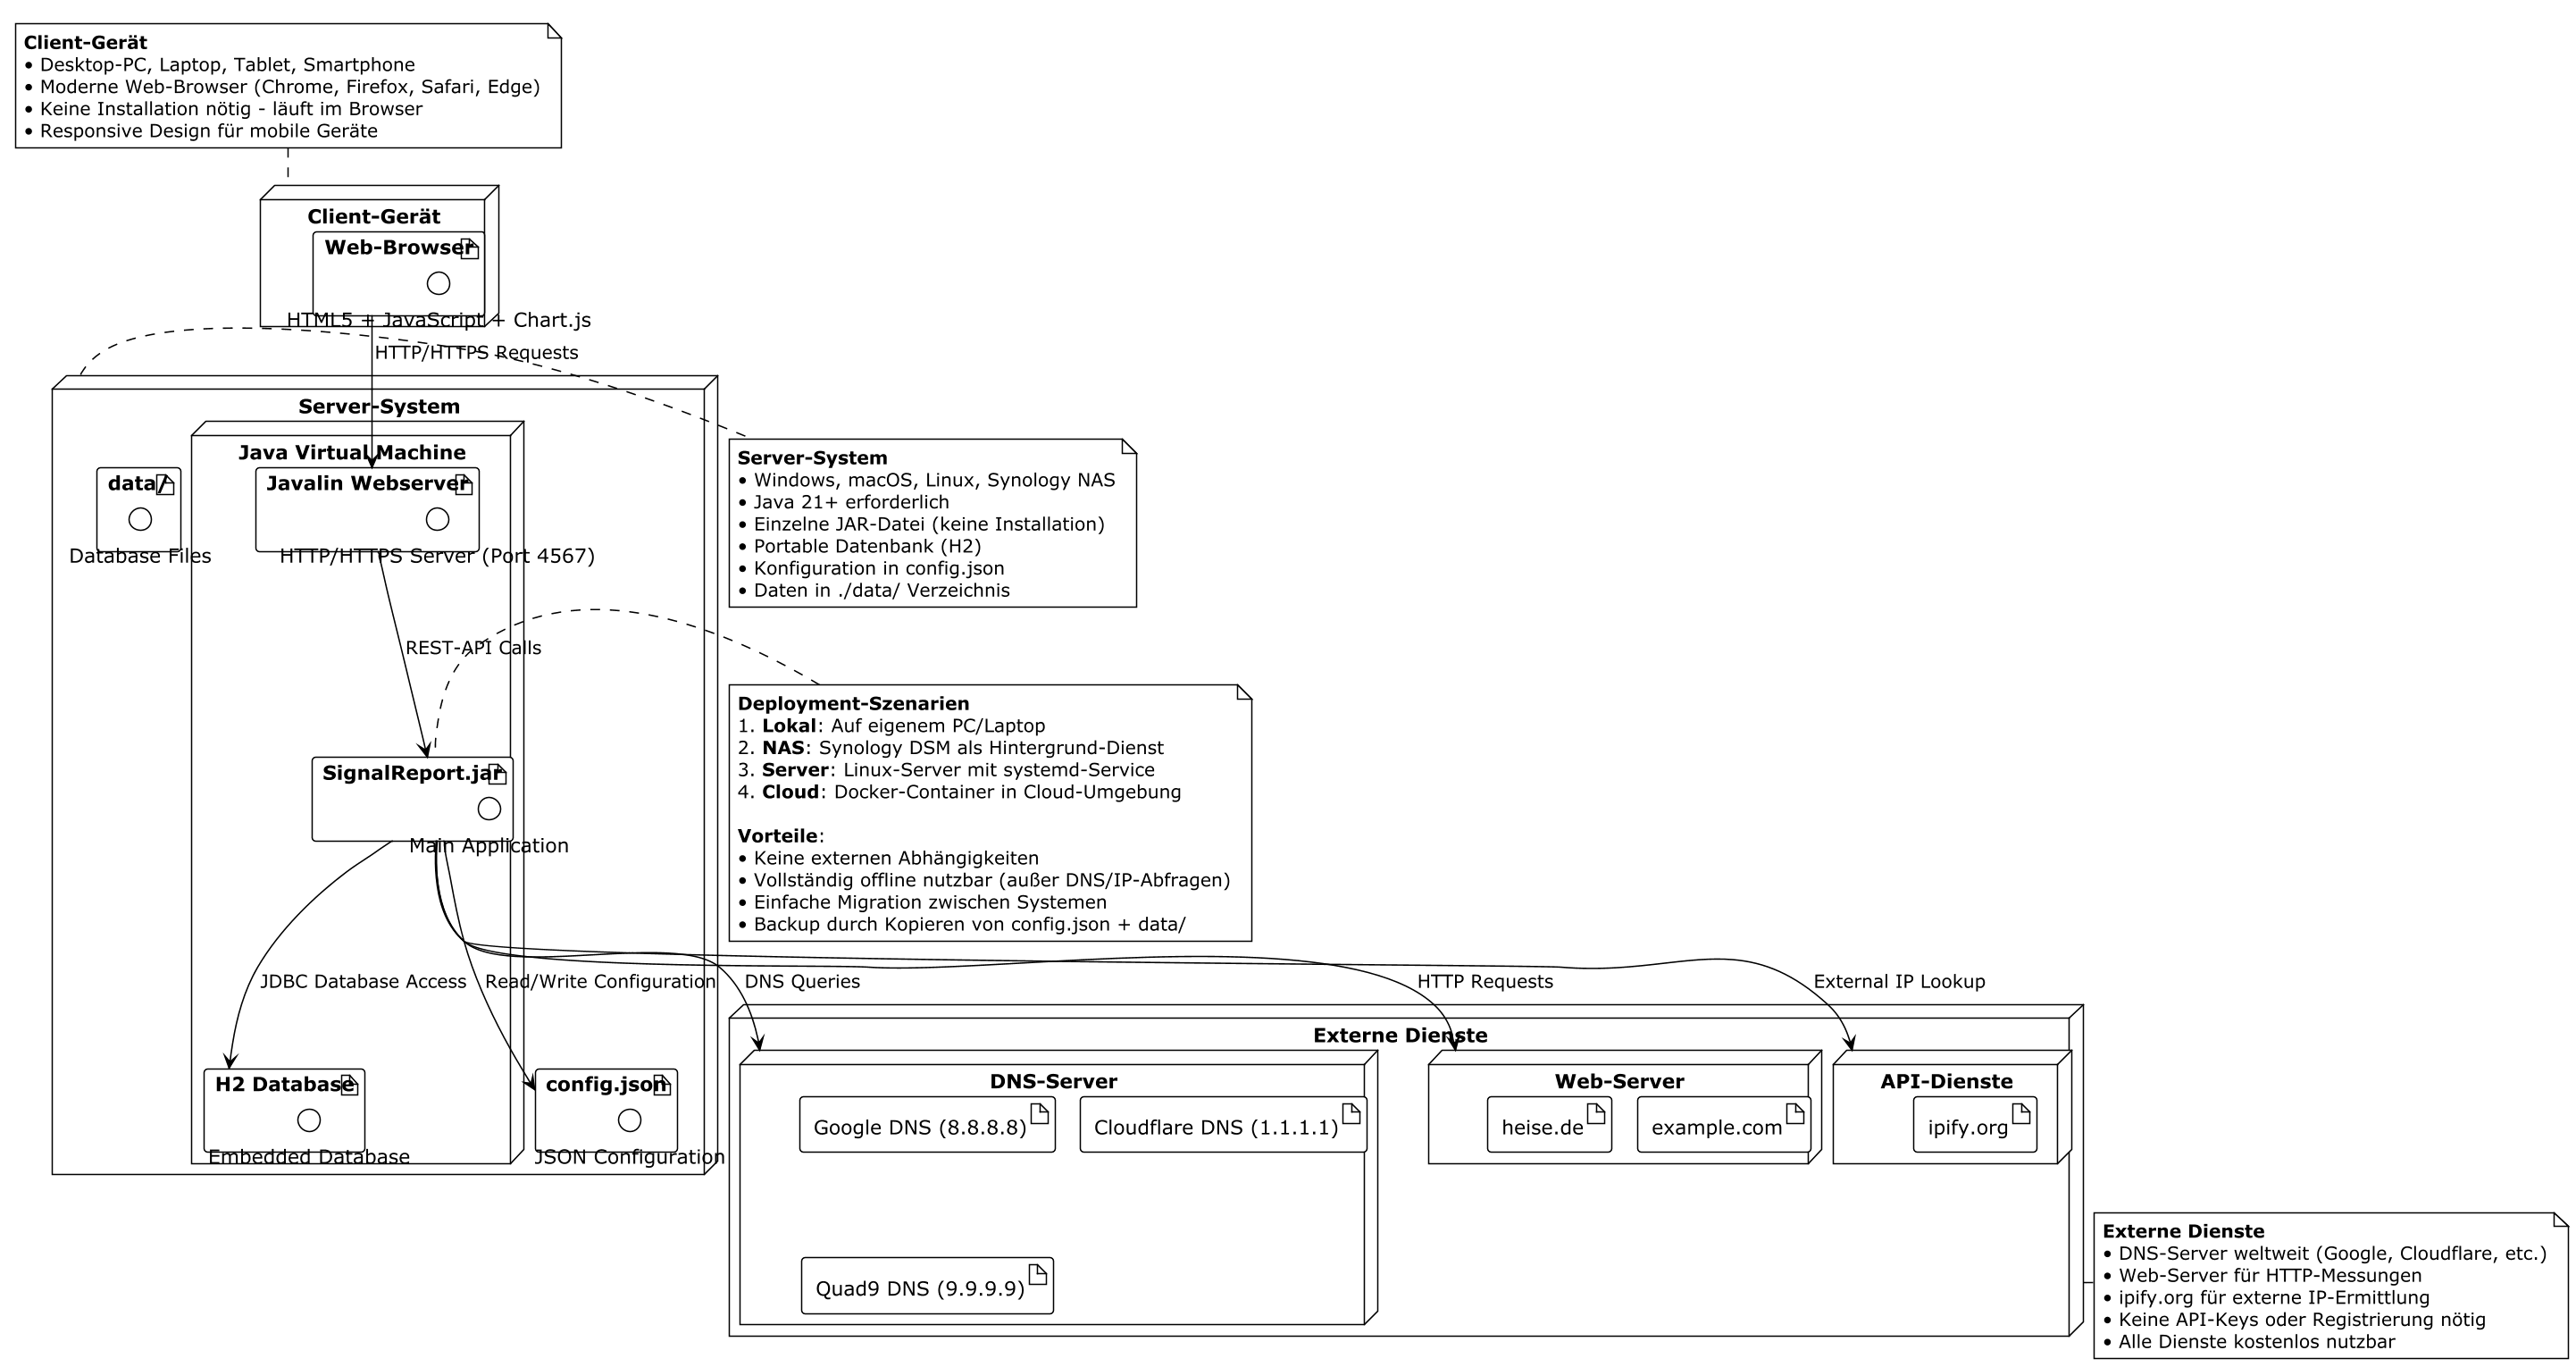
\includegraphics[width=\textwidth]{../diagrams/deployment-diagram.png}
    \caption{Deployment-Diagramm von SignalReport}
    \label{fig:deployment}
\end{figure}

\subsection{Komponenten-Design}

Die Anwendung gliedert sich in sieben Haupt-Packages (Abbildung \ref{fig:component}):

\begin{description}
  \item[measurement] Mess-Engine mit dem \texttt{Measurer}-Interface und drei
    Implementierungen (Ping, DNS, HTTP) sowie dem DNS-Benchmark.
  \item[model] Das \texttt{Measurement}-Datenobjekt als zentrales Transferobjekt.
  \item[persistence] \texttt{H2MeasurementRepository} für die embedded Datenbank
    in Twin-Architektur (Primary + Shadow). Tabellen: Messungen, Hosts, IP-Änderungen.
    Siehe Abschnitt \ref{subsec:twindb}.
  \item[config] Singleton-Konfiguration mit JSON-Persistenz und verschachtelten
    Konfigurations-Klassen (Targets, MaintenanceWindow, Auth, Theme, etc.).
  \item[web] \texttt{WebServer} (Javalin) mit ausgelagertem HTML-Rendering in
    \texttt{HtmlPageRenderer}, \texttt{SetupPageRenderer} und
    \texttt{LoginPageRenderer}. Session-Verwaltung und
    Challenge-Response-Verifikation über \texttt{SessionManager}.
  \item[export] \texttt{PdfReportGenerator} (OpenPDF + JFreeChart) und
    \texttt{PushNotificationService} für Browser-Benachrichtigungen.
  \item[network] \texttt{HostIdentifier} (stabiler Host-Hash) und \texttt{NetworkInfo}
    (lokale/externe IP-Ermittlung).
\end{description}

\begin{figure}[H]
    \centering
    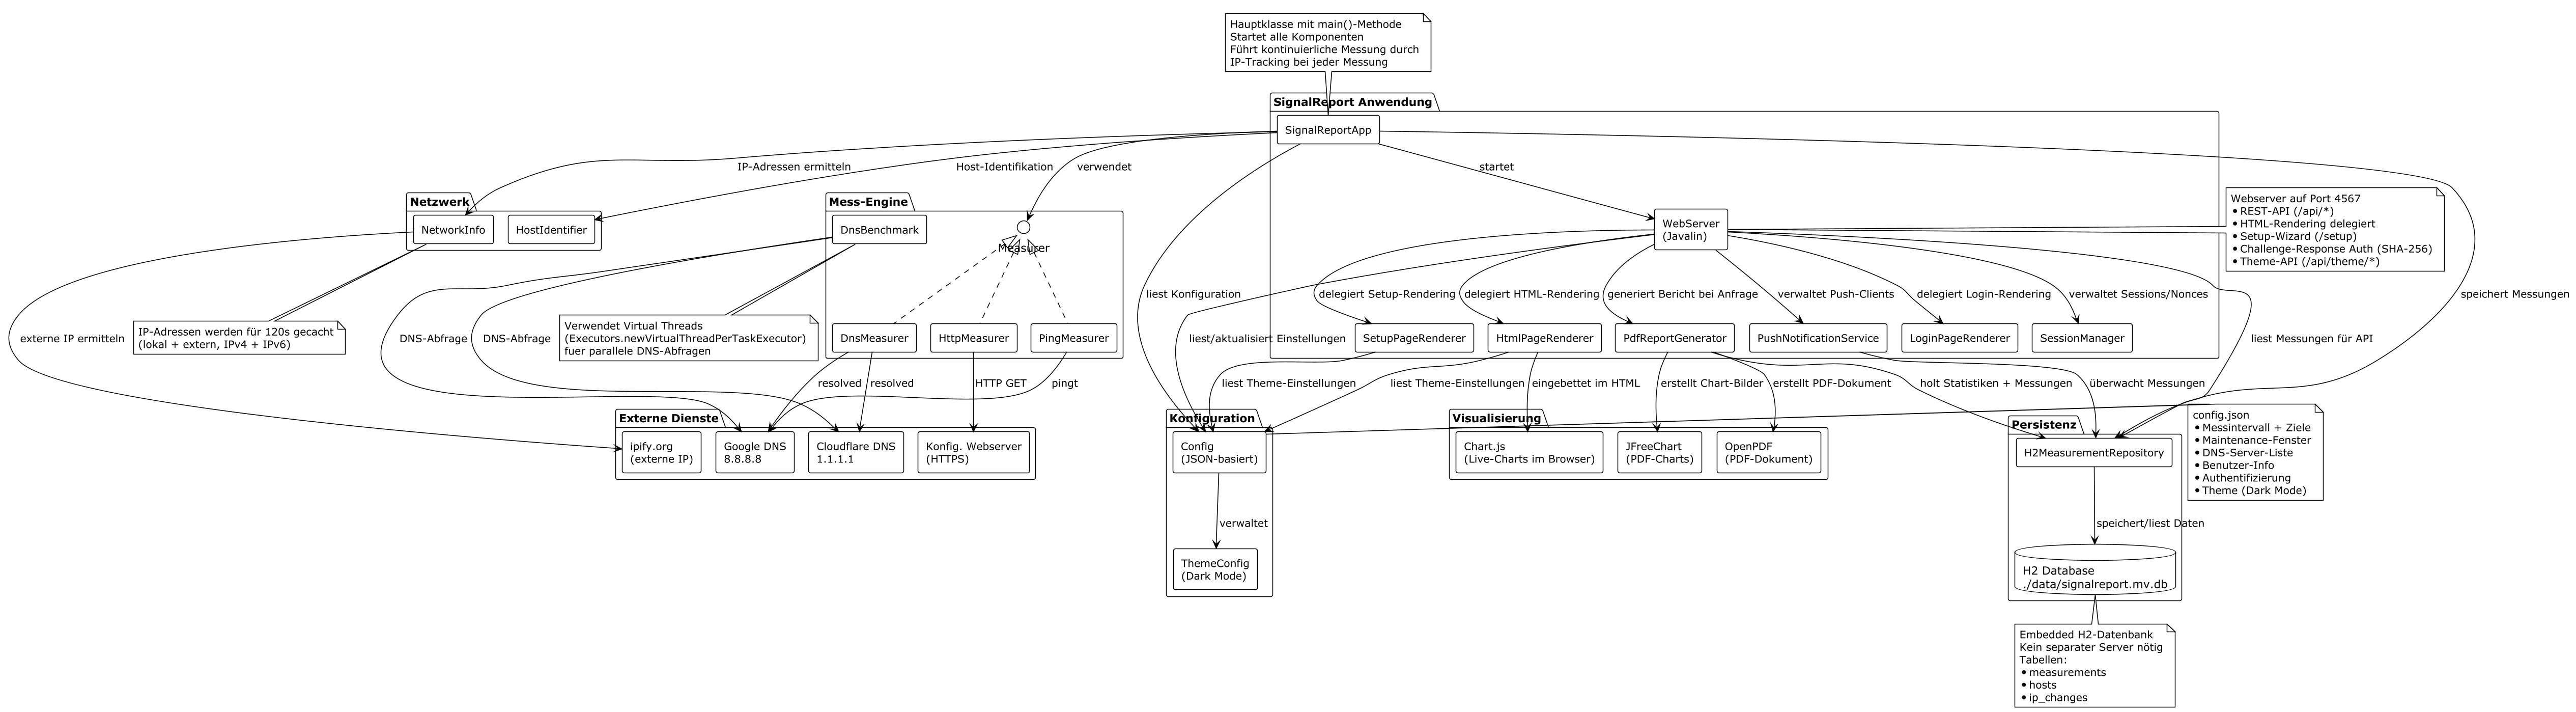
\includegraphics[width=\textwidth]{../diagrams/component-diagram.png}
    \caption{Komponenten-Übersicht von SignalReport}
    \label{fig:component}
\end{figure}

\subsection{Klassen-Design}

Das Klassen-Diagramm in Abbildung \ref{fig:class} zeigt die vollständige Klassenstruktur.
Besonders hervorzuheben sind:

\begin{itemize}
  \item Das \textbf{Measurer-Interface} (Strategy-Pattern): Alle drei Messtypen
    implementieren das gleiche Interface \texttt{Measurer} mit der Methode
    \texttt{measure(String target)}. Dadurch können neue Messtypen hinzugefügt werden,
    ohne bestehenden Code zu ändern (Open/Closed Principle).
  \item Die \textbf{Renderer-Klassen}: Das HTML-Rendering wurde aus dem WebServer in
    eigenständige Klassen ausgelagert (\texttt{HtmlPageRenderer},
    \texttt{SetupPageRenderer}), um die Trennung von Verantwortlichkeiten (Separation of
    Concerns) zu wahren. Der WebServer schrumpfte dadurch von über 2100 auf ca.\ 800
    Zeilen.
  \item Die \textbf{Config-Hierarchie}: Verschachtelte statische Klassen für verschiedene
    Konfigurationsbereiche; zentrale \texttt{hashPassword()}-Methode statt dupliziertem Code.
\end{itemize}

\begin{figure}[H]
    \centering
    
\includegraphics[width=\textwidth]{../diagrams/class-diagram.png}
    \caption{Klassen-Diagramm von SignalReport}
    \label{fig:class}
\end{figure}

\subsection{Design-Entscheidungen}

\begin{table}[h]
\centering
\begin{tabular}{|l|p{9cm}|}
\hline
\textbf{Entscheidung} & \textbf{Begründung} \\
\hline
Monolithische Architektur & Einfachste Installation: eine JAR-Datei, keine externen
  Abhängigkeiten \\
\hline
H2 Embedded Database & Plattformunabhängig, kein separater DB-Server, portable
  Datei \\
\hline
Twin-DB-Architektur & Synchrone Spiegelung in zweite H2-Datei; bei Korruption
  wird die intakte Kopie automatisch zur Reparatur verwendet (vgl.\ Abschnitt \ref{subsec:twindb}) \\
\hline
Javalin statt Spring Boot & Minimaler Overhead (ca.\ 5\,MB vs.\ 30+\,MB), schneller
  Startup \\
\hline
Java 21 & Virtual Threads, Pattern Matching, Text Blocks fuer
  HTML-Templates \\
\hline
OpenPDF statt PDFBox & Einfachere API für Tabellen und Charts; bessere
  Schriftarten-Unterstützung \\
\hline
Inline-HTML statt Templates & Kein Template-Engine-Overhead; Java Text Blocks ermöglichen
  lesbaren HTML-Code; Dark Mode via CSS Custom Properties \\
\hline
Apache Commons Daemon & Professioneller Dienst-Betrieb auf allen Plattformen
  (procrun/jsvc) \\
\hline
\end{tabular}
\caption{Architektur-Entscheidungen (Architecture Decision Records)}
\label{tab:adr}
\end{table}

\subsection{Twin-Datenbank-Architektur}
\label{subsec:twindb}

Nach der Diplomprüfung trat im Produktivbetrieb ein Korruptionsfall der H2-Datenbank
auf, ausgelöst durch einen unvermittelten Windows-Update-Neustart genau während eines
Schreibvorgangs. Die \texttt{.mv.db}-Datei war anschließend nicht mehr lesbar, und auch
das offizielle H2-Recovery-Tool konnte keinen einzigen konsistenten Chunk mehr finden.
Die historischen Messdaten waren damit unwiederbringlich verloren.

Daraufhin wurde die Persistenzschicht von einer einzelnen H2-Datenbank auf eine
\textbf{Twin-Architektur} mit zwei parallel geführten H2-Dateien umgestellt:

\begin{itemize}
  \item \textbf{Primary} (\texttt{signalreport.mv.db}): autoritative Quelle für alle
    Lese-Operationen.
  \item \textbf{Shadow} (\texttt{signalreport-shadow.mv.db}): synchrone Spiegelung
    aller Schreiboperationen.
\end{itemize}

Jede Schreiboperation (\texttt{save}, \texttt{registerHost}, \texttt{recordIpChange})
wird über einen zentralen \texttt{writeOnBoth(\dots)}-Helper sequenziell auf beide
Connections angewendet -- zuerst auf die Primary, danach auf die Shadow. Lese-Operationen
gehen ausschließlich auf die Primary, was den Performance-Overhead minimiert.

\paragraph{Schutz-Stufen.} Drei zusammenwirkende Mechanismen sorgen für Robustheit
gegen abrupte Prozess-Terminierungen (Stromausfall, Update-Neustart, kill -9):

\begin{enumerate}
  \item \texttt{WRITE\_DELAY=0} im JDBC-URL: Jede Transaktion wird synchron auf die
    Platte geflusht (statt Default 500\,ms). Damit verkleinert sich das Korruptions-Fenster
    von Hunderten von Millisekunden auf wenige Mikrosekunden.
  \item \textbf{Twin-Spiegelung}: Selbst wenn eine der beiden Dateien während eines
    Schreibvorgangs zerstört wird, bleibt die jeweils andere konsistent.
  \item \textbf{Auto-Recovery beim Start}: Erkennt der Konstruktor von
    \texttt{H2MeasurementRepository} eine Korruption (H2-Fehlercode 90030), wird die
    defekte Datei in ein \texttt{quarantine/}-Unterverzeichnis verschoben und per
    \texttt{Files.copy()} aus der intakten DB rekonstruiert. Anschließend werden beide
    Connections normal geöffnet -- der Betrieb läuft unterbrechungsfrei weiter.
\end{enumerate}

\paragraph{Fehlerszenarien.} Die Tabelle \ref{tab:twindb-szenarien} dokumentiert das
Verhalten bei den verschiedenen Krisenfällen:

\begin{table}[H]
\centering
\begin{tabular}{|p{5cm}|p{9cm}|}
\hline
\textbf{Szenario} & \textbf{Verhalten} \\
\hline
Crash während Primary-Write & Primary korrupt, Shadow intakt $\to$
  Beim Neustart wird die Primary aus der Shadow rekonstruiert; maximaler Datenverlust:
  die Schreibvorgänge der letzten Sekunden auf die Shadow \\
\hline
Crash während Shadow-Write & Shadow korrupt, Primary intakt $\to$
  Beim Neustart wird die Shadow aus der Primary rekonstruiert; kein Datenverlust \\
\hline
Beide DBs korrupt & Extrem unwahrscheinlich (erfordert Filesystem-Schaden) $\to$
  Beide Dateien werden in Quarantäne verschoben, Betrieb startet mit leeren
  Datenbanken neu, Anwendung bleibt funktional \\
\hline
Shadow-Korruption zur Laufzeit & Sehr selten; Shadow wird deaktiviert, Primary
  läuft weiter, beim nächsten Neustart wird die Shadow automatisch repariert \\
\hline
\end{tabular}
\caption{Twin-DB-Verhalten bei Korruptionsfällen}
\label{tab:twindb-szenarien}
\end{table}

\paragraph{Migration bestehender Installationen.} Existiert beim Update auf die neue
Version bereits eine alte Single-DB ohne Shadow, wird im ersten Konstruktor-Aufruf
die Shadow als exakte Kopie der Primary angelegt. Damit greift die Twin-Redundanz
sofort -- ohne Datenverlust und ohne manuelle Migrationsschritte.

\subsection{Internationalisierung (i18n)}
\label{subsec:i18n}

Die gesamte Präsentationsschicht -- Web-Oberfläche, Login- und Setup-Seite,
PDF-Berichte, CSV-Spaltenköpfe und benutzerseitige API-Meldungen -- ist
mehrsprachig. Aktuell werden neun Sprachen mitgeliefert: Deutsch (Referenz),
Englisch, Französisch, Italienisch, Spanisch, Portugiesisch, Türkisch, Polnisch
und Ukrainisch.

\paragraph{Sprachdateien.} Jede Sprache ist eine flache JSON-Datei (UTF-8) mit
Punkt-Schlüsseln unter \texttt{resources/lang/}, z.\,B.
\texttt{"nav.settings": "Einstellungen"}. Die zentrale Klasse \texttt{I18n}
lädt die in der Konfiguration hinterlegte Sprache und stellt drei Mechanismen
bereit:

\begin{enumerate}
  \item \textbf{Platzhalter-Auflösung}: Die HTML-Renderer enthalten statt
    deutscher Literale Platzhalter der Form \texttt{\{\{nav.settings\}\}}.
    \texttt{I18n.resolve()} ersetzt sie beim Rendern per regulärem Ausdruck.
  \item \textbf{JS-Injektion}: Texte, die das Frontend-JavaScript zur Laufzeit
    erzeugt (Status-Badges, Chart-Beschriftungen, Fehlermeldungen), werden als
    \texttt{const I18N = \{...\}}-Objekt in die Seite eingebettet. Datums- und
    Zahlenformate folgen über die mitgereichte Locale der gewählten Sprache.
  \item \textbf{Direkte Aufrufe}: PDF-Generator und WebServer verwenden
    \texttt{I18n.get(key)} sowie locale-bewusste Formatierung
    (\texttt{String.format(locale, ...)}) -- im Deutschen erscheint
    \texttt{23,5 ms}, im Englischen \texttt{23.5 ms}.
\end{enumerate}

\paragraph{Fallback-Kette.} Fehlt ein Schlüssel in der gewählten Sprache, wird
auf Deutsch (Referenzsprache) zurückgegriffen, danach auf den Schlüsselnamen
selbst -- die Oberfläche zeigt also nie ein Loch. Ein eigener Testfall
(\texttt{I18nTest}) erzwingt zusätzlich, dass alle mitgelieferten Sprachdateien
exakt dieselben Schlüssel wie die Referenz enthalten und dass jeder im
Quellcode verwendete Platzhalter existiert.

\paragraph{Erweiterbarkeit ohne Neukompilieren.} Neben den im JAR gebündelten
Sprachen liest \texttt{I18n} einen externen Ordner \texttt{./lang} neben der
JAR-Datei ein. Eine dort abgelegte Datei (z.\,B. \texttt{ca.json} für
Katalanisch) erscheint automatisch im Sprach-Dropdown; gleichnamige Dateien
überschreiben gebündelte Sprachen, womit auch Übersetzungskorrekturen ohne
Neubau möglich sind. Der Anzeigename jeder Sprache stammt aus ihrem eigenen
Schlüssel \texttt{language.name} und erscheint im Dropdown in der jeweiligen
Eigenbezeichnung (Deutsch, English, Türkçe, Ukrainisch in kyrillischer
Schrift usw.).

\paragraph{Sprachwahl.} Die Sprache wird global pro Installation in
\texttt{config.json} gespeichert. Sie ist an zwei Stellen umstellbar: per
Dropdown im Setup-Wizard (noch vor der Passwortvergabe, via
\texttt{/setup?lang=xx}) und im Einstellungen-Tab (sofortige Übernahme über
\texttt{POST /api/config/language} mit anschließendem Seiten-Reload).
Neuinstallationen starten in der Systemsprache des Rechners, sofern
unterstützt -- andernfalls auf Englisch. Bestehende Konfigurationen ohne
\texttt{language}-Feld bleiben unverändert auf Deutsch.

\paragraph{PDF und Sonderzeichen.} Die eingebauten PDF-Schriften (Helvetica)
beherrschen nur Westeuropa-Zeichen; Türkisch, Polnisch und Ukrainisch wären
damit im Bericht nicht darstellbar. Deshalb wird die freie Schrift
\textbf{DejaVu Sans} (Regular, Bold, Oblique) als Ressource mitgeliefert und
mit Unicode-Encoding (\texttt{IDENTITY\_H}) in jedes PDF eingebettet. Dieselben
TTF-Dateien dienen JFreeChart als AWT-Schrift, sodass auch Chart-Titel und
Achsenbeschriftungen in allen Sprachen korrekt gerendert werden. Der
JAR-Zuwachs durch Schriften und neun Sprachdateien beträgt rund 1,5\,MB.

\subsection{Datenfluss bei der Messung}

Der Messablauf (Abbildung \ref{fig:sequence-measurement}) zeigt den kontinuierlichen
Zyklus:
\begin{enumerate}
  \item Konfiguration laden und Maintenance-Fenster prüfen
  \item Externe IP ermitteln und IP-Änderungen protokollieren
  \item Drei Messungen ausführen (Ping, DNS, HTTP)
  \item Ergebnisse in der Datenbank speichern
  \item Konfigurierbares Intervall abwarten
\end{enumerate}

\begin{figure}[H]
    \centering
    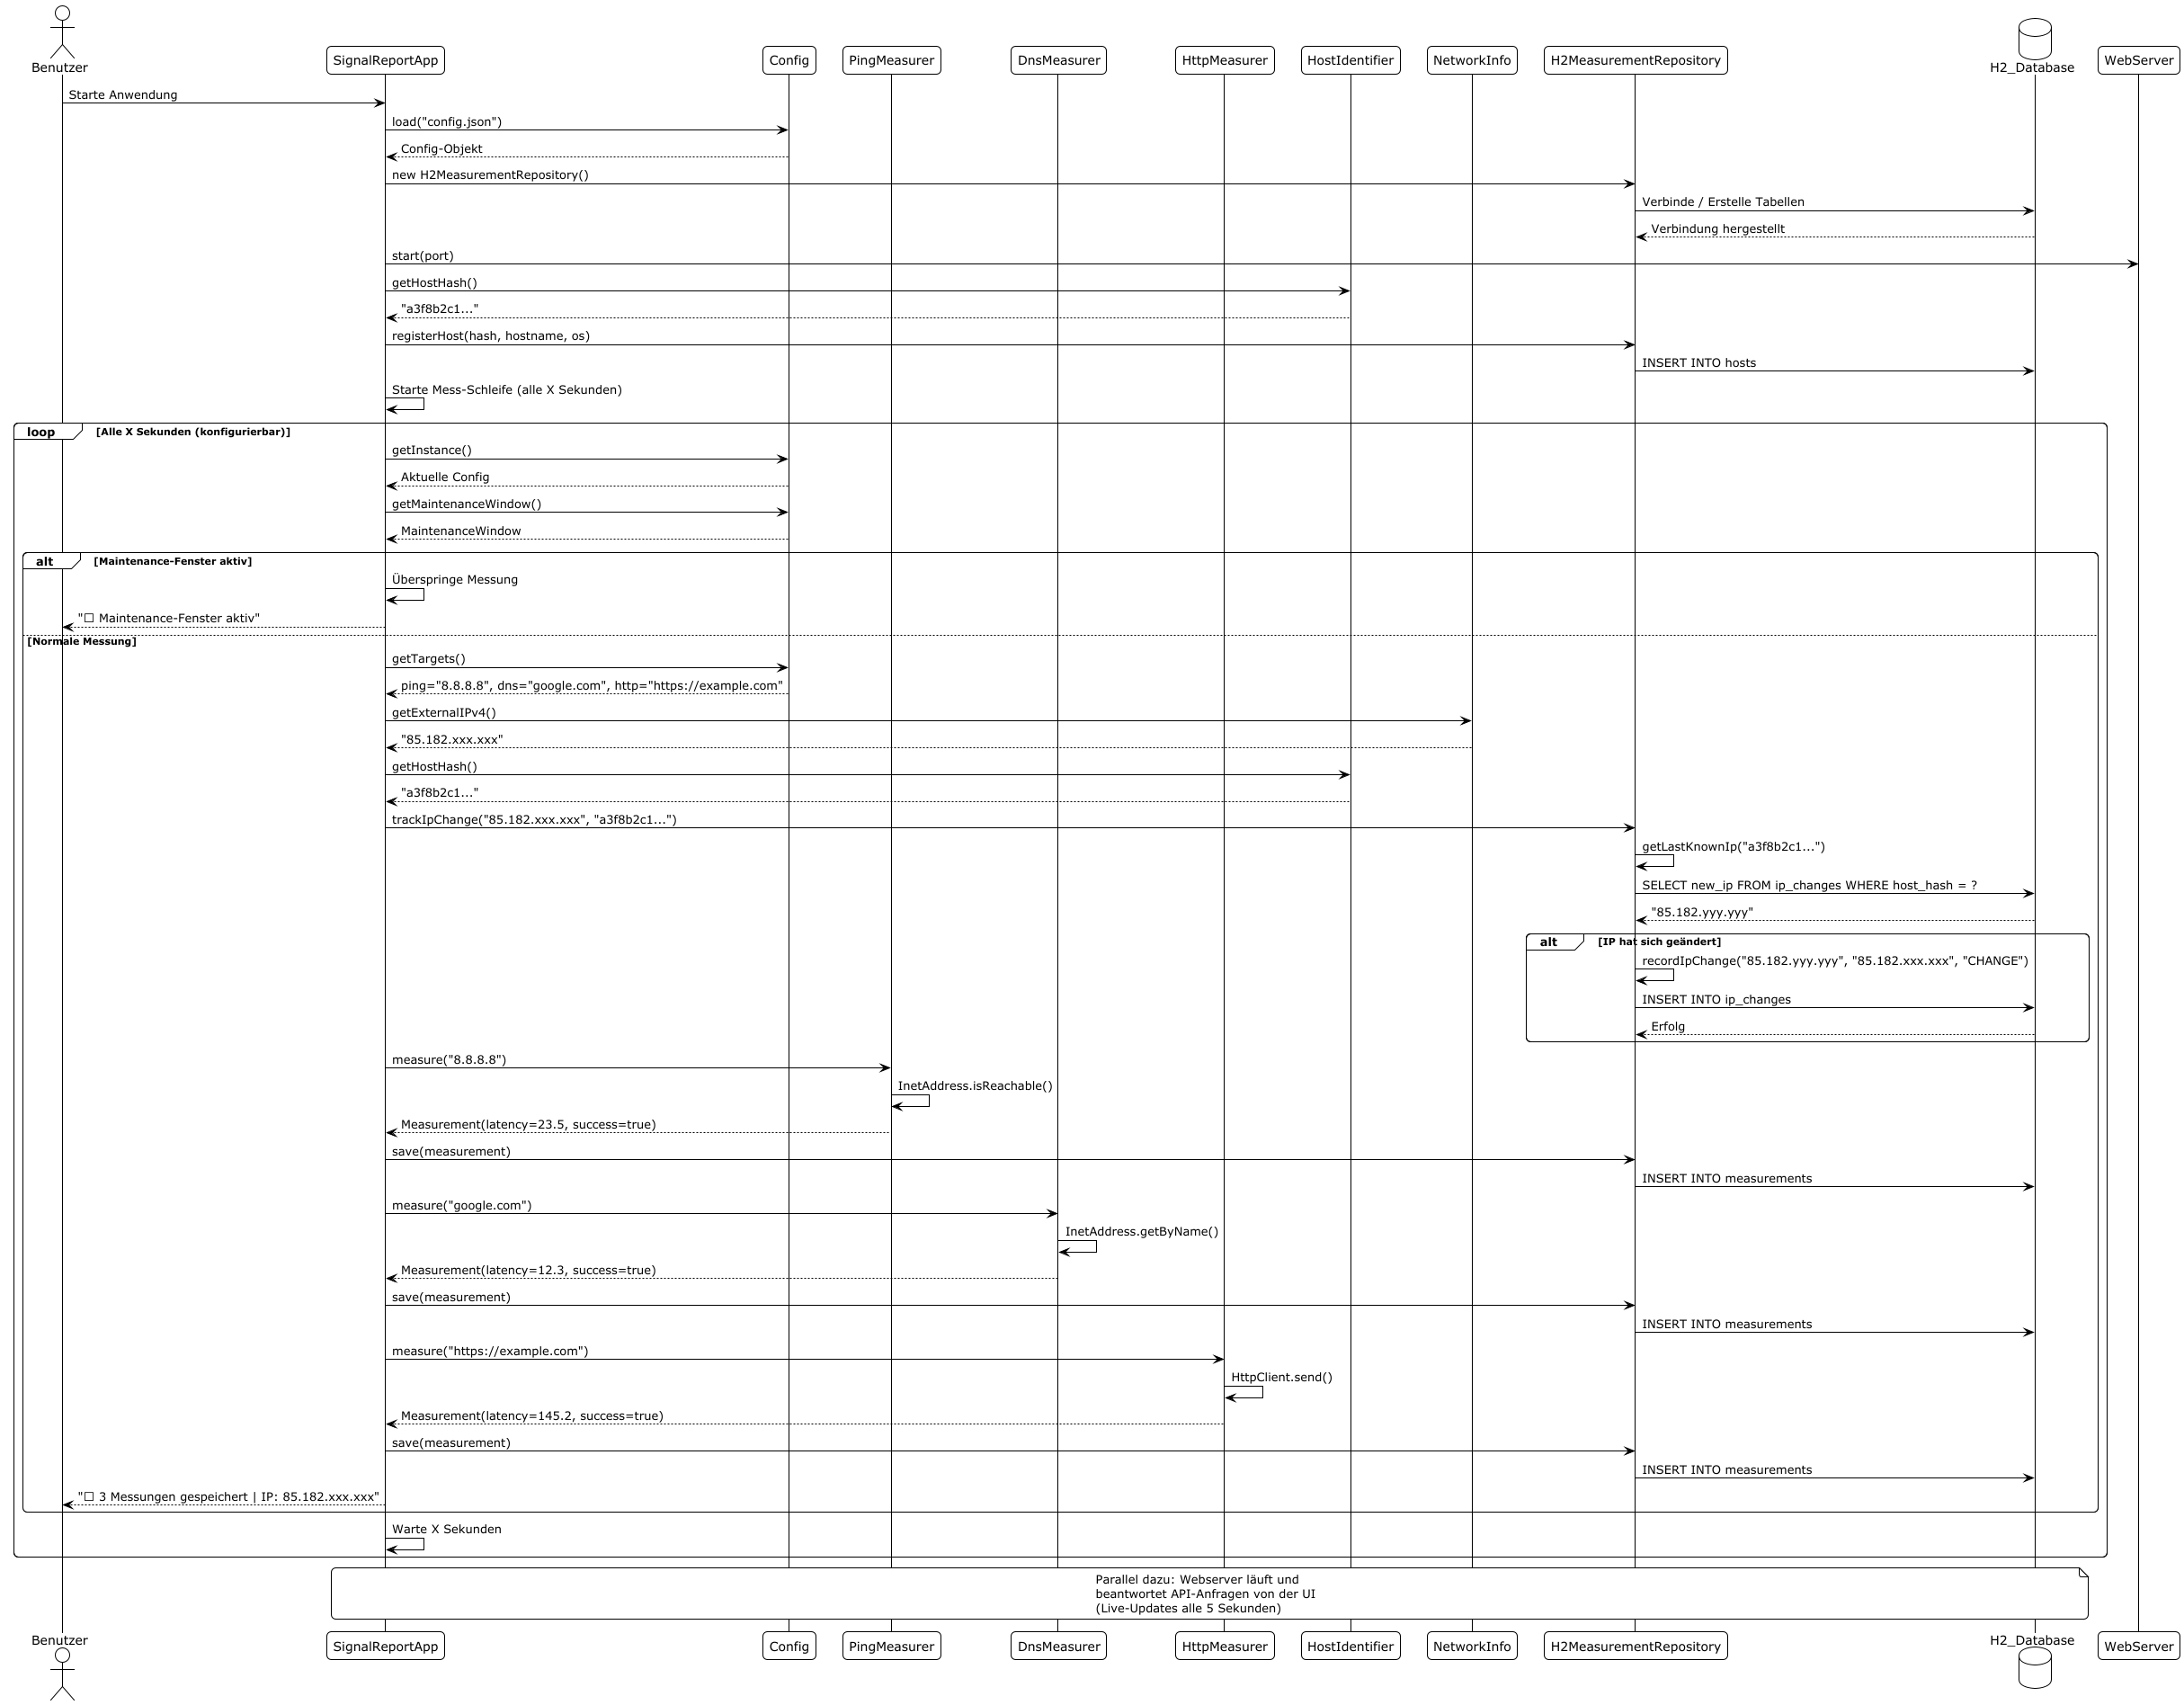
\includegraphics[width=\textwidth]{../diagrams/sequence-measurement.png}
    \caption{Sequenzdiagramm: Messablauf}
    \label{fig:sequence-measurement}
\end{figure}

\subsection{PDF-Export-Prozess}

Der PDF-Bericht (Abbildung \ref{fig:sequence-pdf}) durchläuft mehrere Schritte:
Statistik-Berechnung, Chart-Generierung mit JFreeChart, Zieländerungs-Erkennung,
Ausfall-Analyse und abschliessende PDF-Zusammenstellung mit OpenPDF.

\begin{figure}[H]
    \centering
    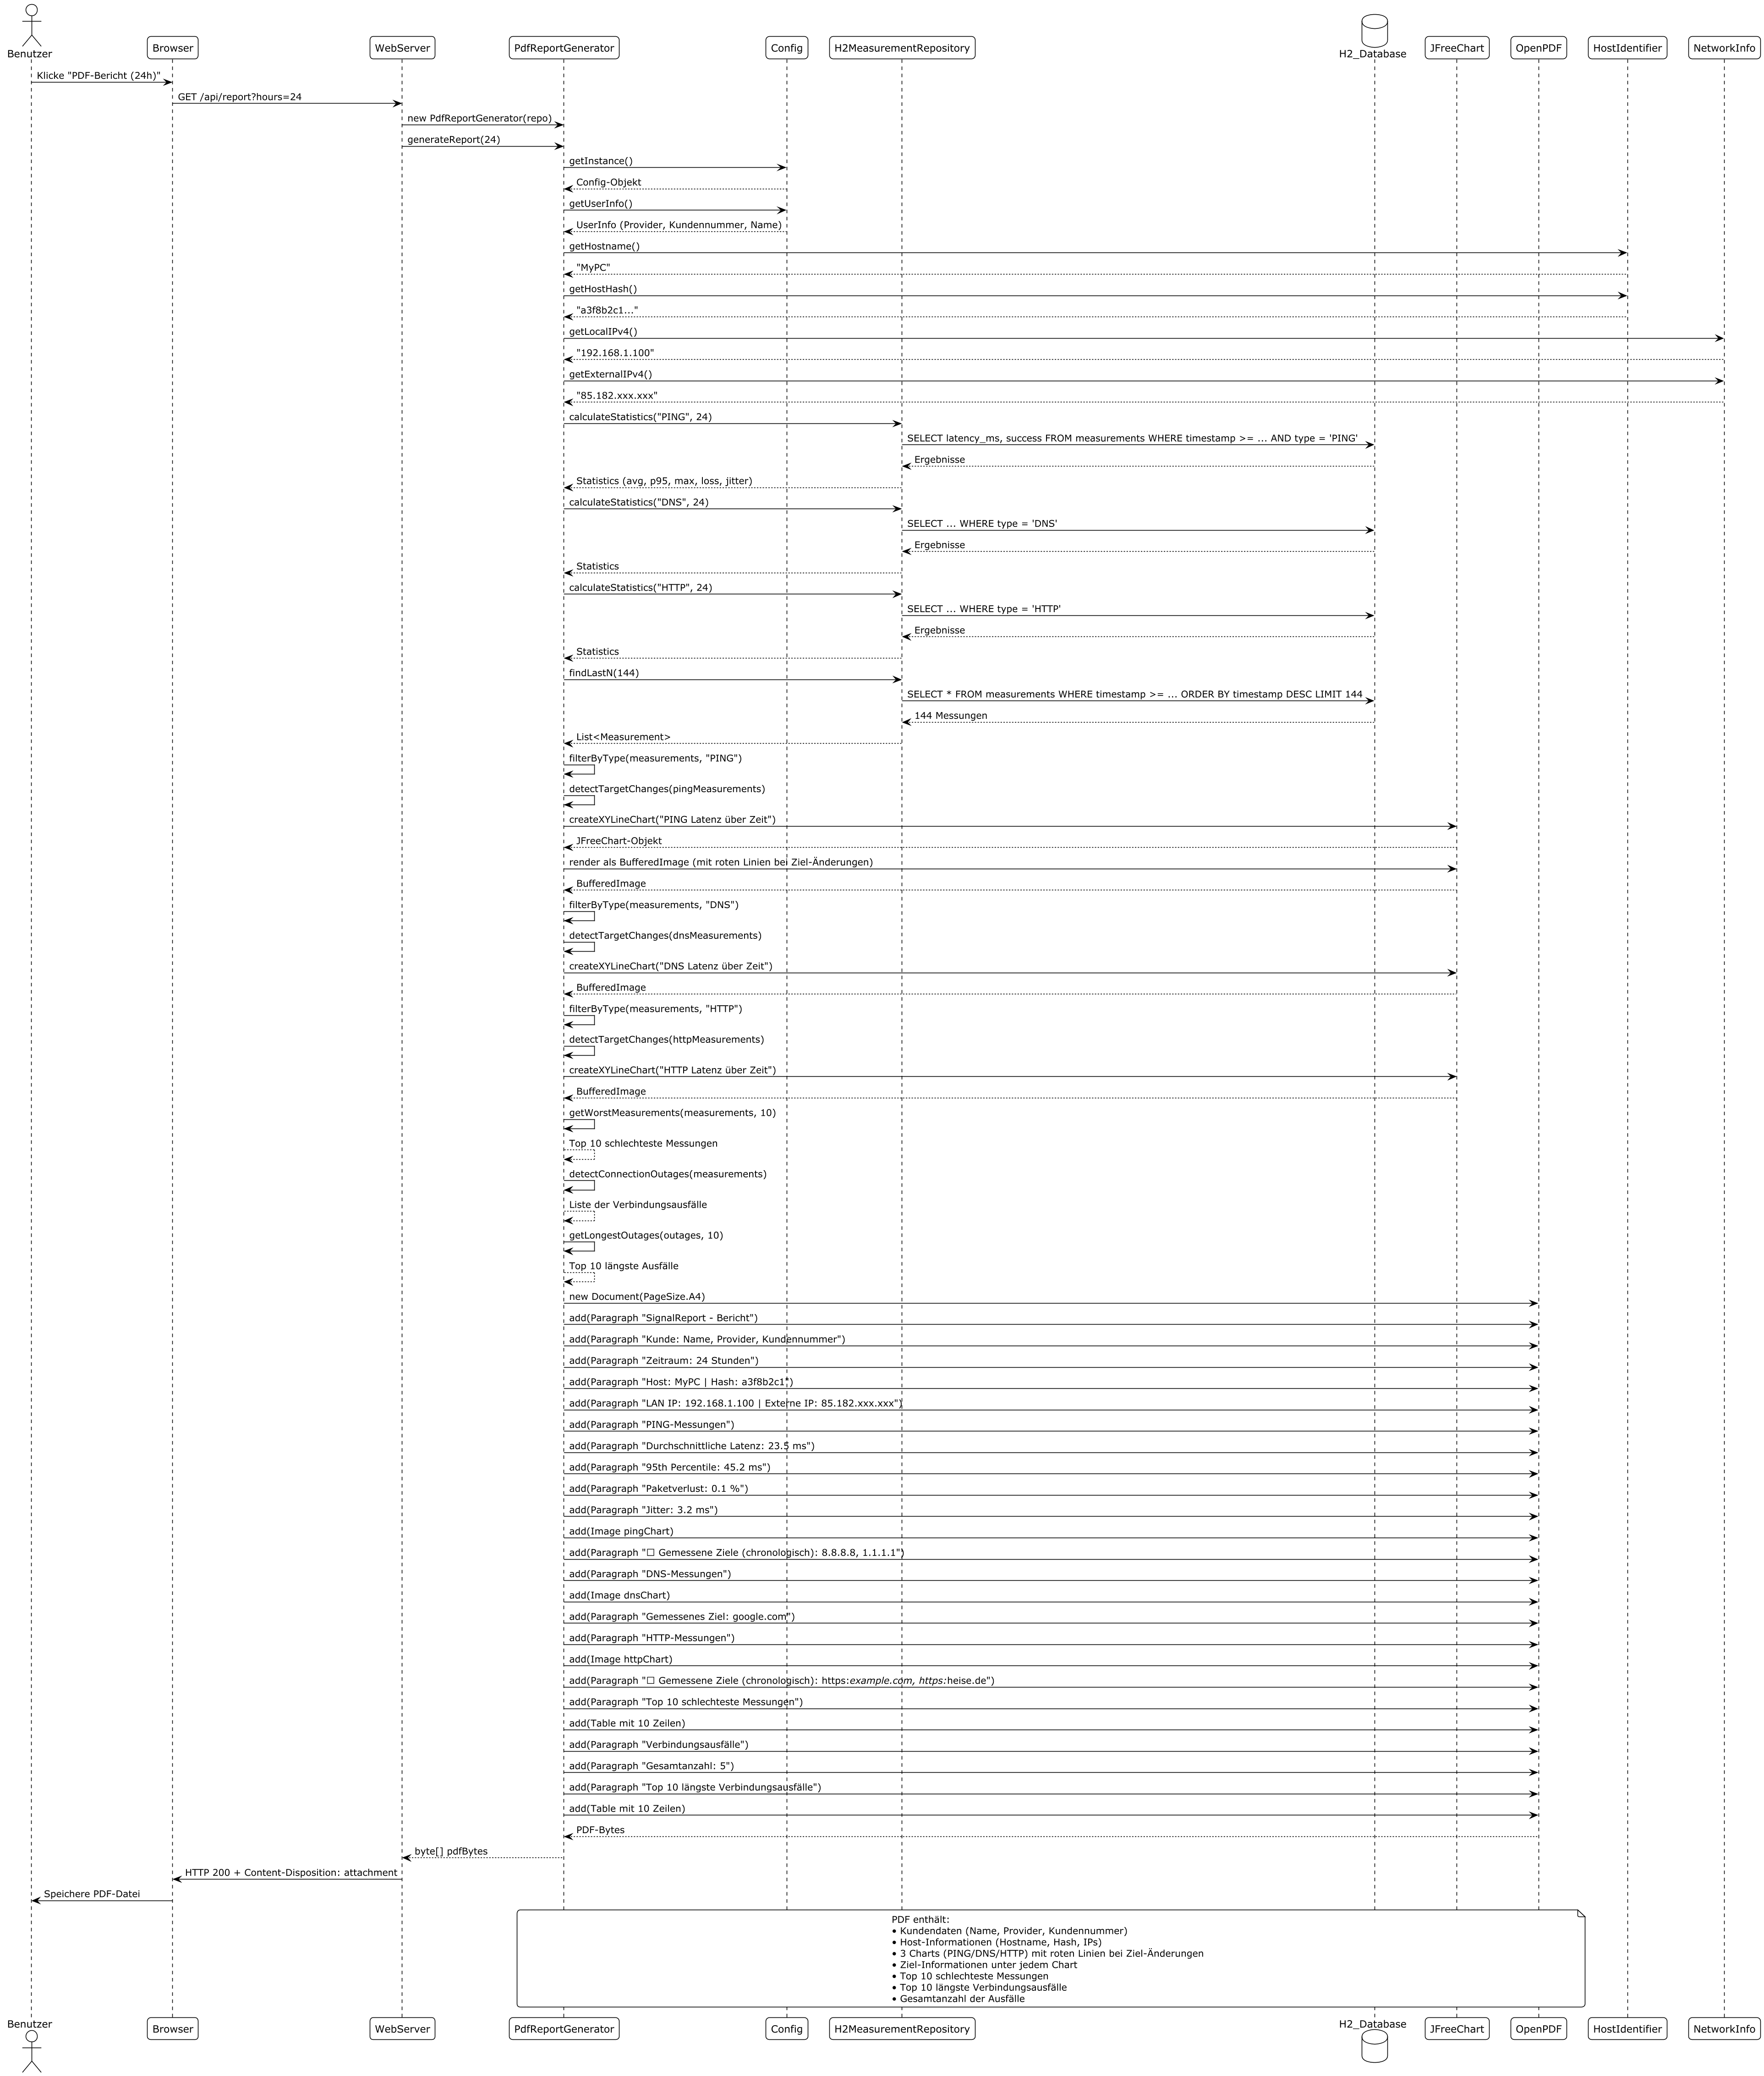
\includegraphics[width=\textwidth]{../diagrams/sequence-pdf.png}
    \caption{Sequenzdiagramm: PDF-Export}
    \label{fig:sequence-pdf}
\end{figure}

\subsection{Use-Cases}

Das Use-Case-Diagramm (Abbildung \ref{fig:usecase}) zeigt alle 16 Anwendungsfälle,
aufgeteilt auf die drei Akteure Benutzer, Administrator und System. Die vollständigen
User Stories zu jedem Use Case finden sich in Abschnitt \ref{sec:userstories}.

\begin{figure}[H]
    \centering
    
\includegraphics[width=0.9\textwidth]{../diagrams/usecase-diagram.png}
    \caption{Use-Case-Diagramm von SignalReport}
    \label{fig:usecase}
\end{figure}

\subsection{Authentifizierungs-Zustände}

Das State-Diagramm (Abbildung \ref{fig:state-auth}) modelliert den Lebenszyklus der
Authentifizierung: vom initialen Setup über den öffentlichen Zugriff bis zum geschützten
Modus mit Admin- und User-Rollen.

\begin{figure}[H]
    \centering
    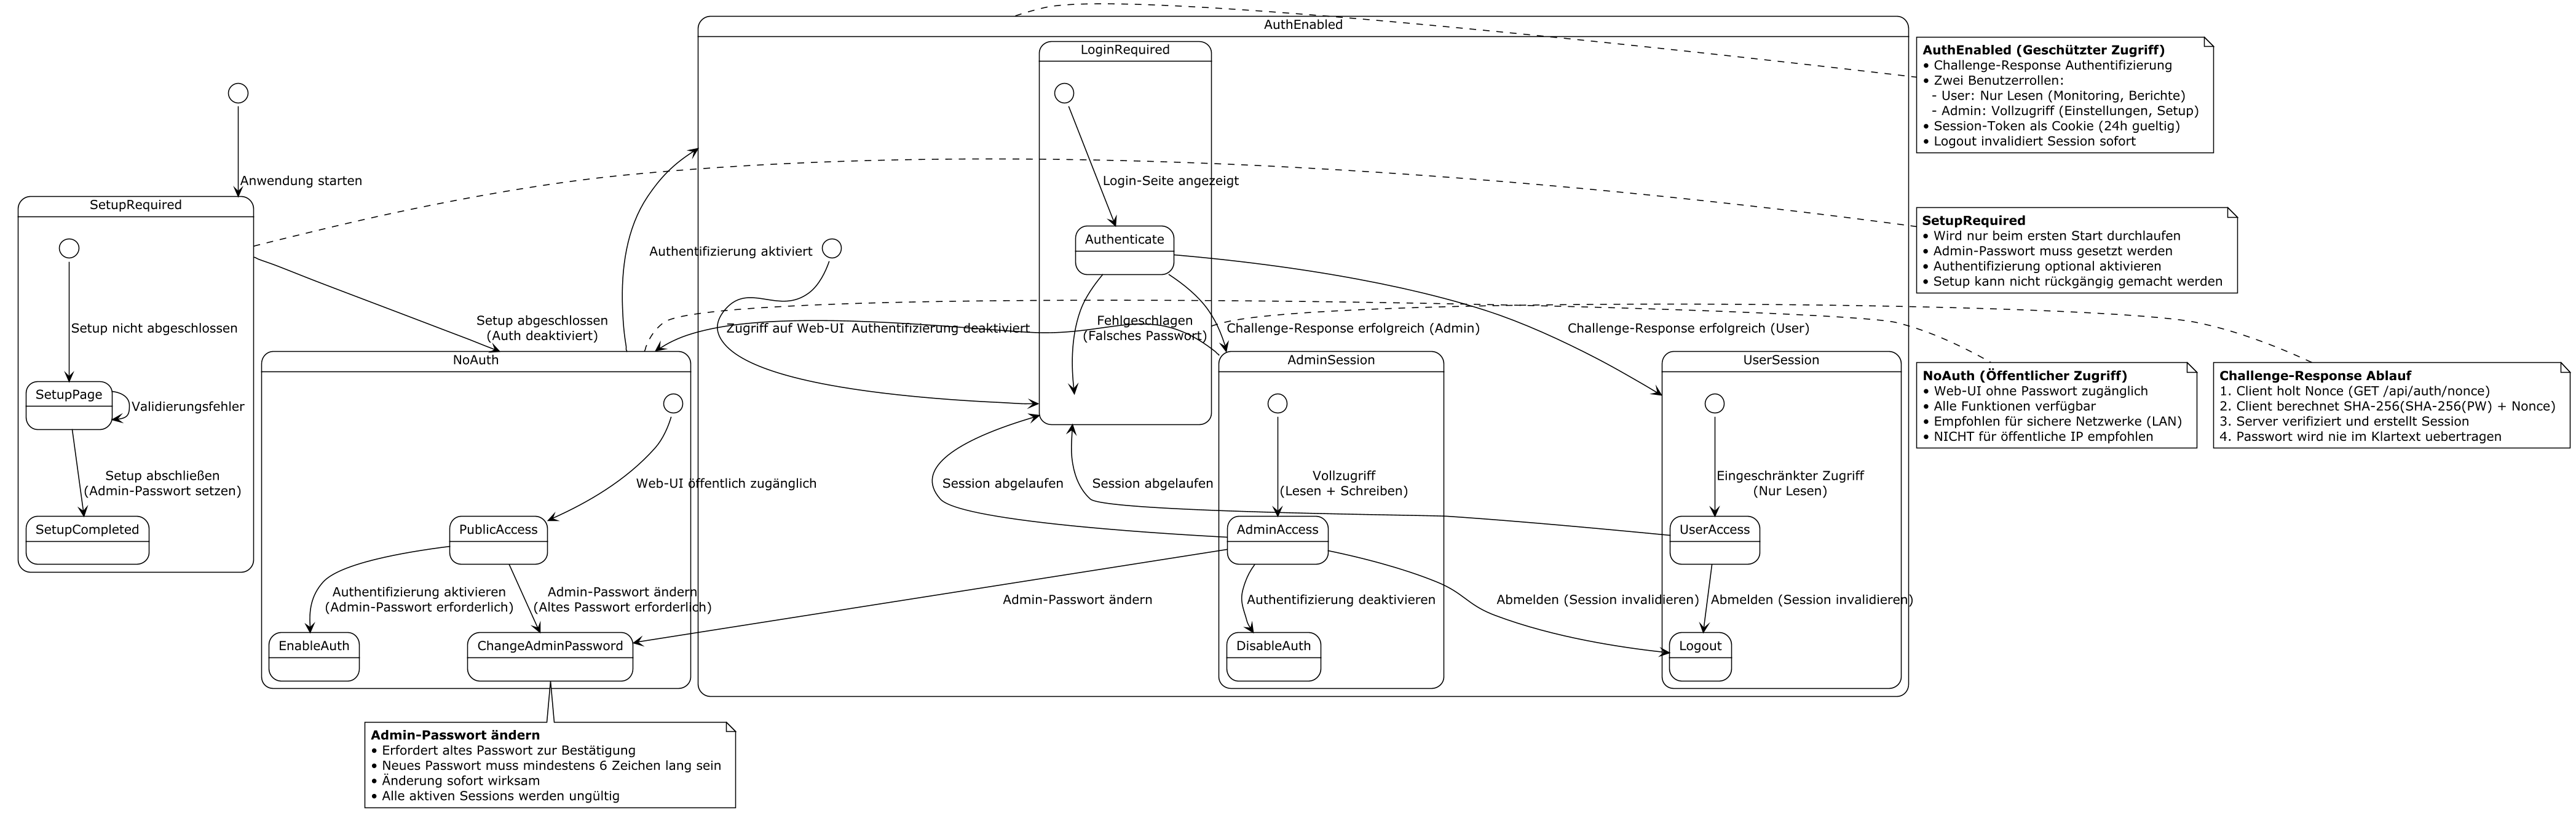
\includegraphics[width=0.9\textwidth]{../diagrams/state-diagram-auth.png}
    \caption{State-Diagramm: Authentifizierung}
    \label{fig:state-auth}
\end{figure}


% Kapitel 4: Implementierung
\section{Implementierung}
\label{sec:implementierung}

\subsection{Mess-Engine}
Die Mess-Engine implementiert drei Messarten:

\begin{itemize}
    \item \textbf{Ping-Messung}: Nutzt \texttt{InetAddress.isReachable()}
    \item \textbf{DNS-Messung}: Nutzt \texttt{InetAddress.getByName()}
    \item \textbf{HTTP-Messung}: Nutzt \texttt{java.net.http.HttpClient}
\end{itemize}

\begin{lstlisting}[language=Java, caption=Beispiel für Ping-Messung]
public Measurement measure() throws Exception {
    long start = System.nanoTime();
    boolean reachable = InetAddress.getByName(target).isReachable(3000);
    long end = System.nanoTime();
    double latency = (end - start) / 1_000_000.0;
    return new Measurement(target, latency, reachable, "PING");
}
\end{lstlisting}

\subsection{Statistische Auswertung}
Die statistische Auswertung berechnet folgende Kennzahlen:

\begin{itemize}
    \item \textbf{Durchschnittliche Latenz}: $\mu = \frac{1}{n}\sum_{i=1}^{n}x_i$
    \item \textbf{95th Percentile}: Wert, unter dem 95\% der Messungen liegen
    \item \textbf{Paketverlust}: $\frac{\text{fehlgeschlagene Messungen}}{\text{gesamte Messungen}} \times 100$
    \item \textbf{Jitter}: Durchschnitt der Differenzen zwischen aufeinanderfolgenden Messungen
\end{itemize}

\begin{lstlisting}[language=Java, caption=Beispiel für 95th Percentile-Berechnung]
// Statistiken aus der Datenbank holen
List<Double> latencies = new ArrayList<>();
// ... Daten laden ...
Collections.sort(latencies);
int p95Index = (int) Math.ceil(latencies.size() * 0.95) - 1;
double p95Latency = latencies.get(p95Index);
\end{lstlisting}

\subsection{Web-Interface}
Das Web-Interface wurde mit Javalin implementiert:

\begin{itemize}
    \item \textbf{REST-API}: Für Datenzugriff (z. B. \texttt{/api/measurements})
    \item \textbf{Live-Chart}: Aktualisiert sich alle 5 Sekunden
    \item \textbf{Heatmap}: Zeigt Latenzentwicklung pro Stunde
    \item \textbf{Statistik-Panel}: Sofortige Einschätzung der Netzwerkqualität
\end{itemize}

\begin{figure}[H]
    \centering
    \includegraphics[width=0.8\textwidth]{../diagrams/ui.png}
    \caption{Web-Interface von SignalReport}
    \label{fig:ui}
\end{figure}

% Kapitel 5: Test
\section{Test}
\label{sec:test}

\subsection{Teststrategie}
Die Teststrategie umfasste:

\begin{itemize}
    \item \textbf{Unit-Tests}: Für die Kernkomponenten (z. B. Statistik-Berechnung, Config-Handling, Measurer-Interface)
    \item \textbf{Integrationstests}: Für die Datenbankanbindung und API-Endpunkte
    \item \textbf{E2E-Tests}: Für das Web-Interface und PDF-Export
    \item \textbf{Manuelle Tests}: Für UI-Interaktionen und Benutzerfreundlichkeit
\end{itemize}

\subsection{JUnit-Testabdeckung}
SignalReport wurde mit JUnit 5 umfassend getestet. Die 18 Testklassen mit laufenden Tests -- in Paketen, die die Quellstruktur spiegeln (\texttt{config}, \texttt{measurement}, \texttt{network}, \texttt{storage}, \texttt{report}, \texttt{web}, \texttt{i18n}) -- mit insgesamt 156 Tests (zuzüglich zweier netz- bzw.\ PDF-gebundener Smoke-Klassen, die per Umgebungsvariable aktivierbar sind) decken folgende Bereiche ab:

\begin{itemize}
    \item \textbf{MeasurementTest} (5 Tests): Grundlegende Objekt-Erstellung und Validierung
    \item \textbf{HostIdentifierTest} (4 Tests): Stabile Host-Identifikation über Neustarts
    \item \textbf{StatisticsTest} (8 Tests): Mathematisch korrekte Berechnung von 95. Perzentil, Jitter und Paketverlust mit realen DB-Abfragen
    \item \textbf{ConfigTest} (17 Tests): Laden/Speichern von Konfiguration, hashPassword, Auth-Verifikation, Theme, Save+Reload
    \item \textbf{H2MeasurementRepositoryTest} (10 Tests): Vollstaendige Datenbank-Integration mit IP-Tracking, Host-Registrierung
    \item \textbf{MeasurerInterfaceTest} (6 Tests): Interface-Implementierung, Polymorphie, reale Messungen (Ping/DNS/HTTP)
    \item \textbf{MaintenanceWindowTest} (7 Tests): Deaktiviert, ganztägig, aktuelle Zeit, Mitternachtsübergang, Standardwerte
    \item \textbf{SessionManagerTest} (19 Tests): Nonce-Generierung und -Validierung (Single-Use, Ablauf), Session-Erstellung und -Timeout (24\,h), Rollen\-unter\-schei\-dung (Admin/User), Challenge-Response-Verifikation, Replay-Schutz
    \item \textbf{I18nTest} (10 Tests): Schlüssel-Parität aller neun Sprachdateien gegen die Referenz (de.json), Existenz aller im Quellcode verwendeten Platzhalter (inkl. \texttt{app.js}), Fallback-Verhalten, Sprach-Erkennung
    \item \textbf{GatewayDiscoveryTest} (15 Tests): Traceroute-Parsing, RFC-1918-Klassifizierung, Gateway-Kette (nah/fern), Erkennung virtueller Gateways (Docker-Bridge, VM-NAT) und Überspringen der Docker-Bridge
    \item \textbf{ConnectivityAssessmentTest} (8 Tests): Schuld-Verdikt (Router / Internet-Gateway / Internet) auf Basis des Paketverlusts je Segment
    \item \textbf{ReliabilityReportTest} (10 Tests): lückenbewusste Verfügbarkeit/Abdeckung/MTBF/MTTR, Aggregation aufeinanderfolgender Fehlmessungen zu einem Ausfall, Ausschluss via \texttt{excluded}-Spalte
    \item \textbf{ServiceReachabilityConfigTest} (8 Tests): Defaults (deaktiviert, 6-Stunden-Takt), Intervall-Grenzen, Pro-Dienst-Schalter, JSON-Round-Trip
    \item \textbf{ServiceReachabilityAssessmentTest} (15 Tests): Verdikt-Klassifizierung (erreichbar / Dienst-Störung / DNS-, TCP-, SNI-Sperre / Sperrseite) aus synthetischen Beobachtungen
    \item \textbf{ServiceReachabilityReportTest} (4 Tests): Verdichtung der Prüfungen zu Episoden (die Sperr-/Störungs-Timeline)
    \item \textbf{ServiceReachabilitySchedulerTest} (5 Tests): Leitungs-Gate-Entscheidung (nur erfolgreiche PING-/HTTP-Messungen zählen als Internet-Beleg)
    \item \textbf{ServiceCheckRepositoryTest} (3 Tests): \texttt{service\_checks}-Persistenz, Zeitraum-Abfrage, neueste Prüfung je Dienst
    \item \textbf{ServiceReachabilityRoutesTest} (2 Tests): \enquote{Jetzt prüfen}-Endpoint inkl.\ Abkühlphase (gegen echten Javalin-Server)
\end{itemize}

Alle Tests laufen ohne externe Abhängigkeiten (H2 In-Memory-Datenbanken für Integrationstests) und sind in unter 2 Sekunden durchführbar.

\subsection{Beispiel-Test für Statistik-Berechnung}
\begin{lstlisting}[language=Java, caption=Test fuer 95. Perzentil]
@Test
void testP95CalculationWithSortedLatencies() {
    // Arrange: 20 Messungen (95. Perzentil = 19. Wert)
    List<Double> latencies = new ArrayList<>();
    for (int i = 1; i <= 20; i++) {
        latencies.add((double) i * 10); // 10, 20, 30, ..., 200
    }

    // Act: 95. Perzentil = Index 18 (0-basiert) = 190.0
    int p95Index = (int) Math.ceil(latencies.size() * 0.95) - 1;
    double p95Value = latencies.get(p95Index);

    // Assert
    assertEquals(18, p95Index, "Index fuer 95. Perzentil muss 18 sein");
    assertEquals(190.0, p95Value, 0.01, "95. Perzentil-Wert muss 190.0 sein");
}
\end{lstlisting}

\subsection{Testergebnisse}
\begin{table}[H]
\centering
\small
\begin{tabular}{|p{8.5cm}|l|l|}
\hline
\textbf{Testkategorie} & \textbf{Anzahl} & \textbf{Erfolgsquote} \\
\hline
Unit-Tests (Measurement, HostIdentifier, Config, Measurer, MaintenanceWindow, SessionManager, I18n, GatewayDiscovery, ConnectivityAssessment, ReliabilityReport, ServiceReachabilityConfig, ServiceReachabilityAssessment, ServiceReachabilityReport, ServiceReachabilityScheduler) & 133 & 100\% \\
\hline
Integrationstests (Statistics, H2MeasurementRepository, ServiceCheckRepository, ServiceReachabilityRoutes) & 23 & 100\% \\
\hline
E2E-Tests (manuell: Web-UI, PDF-Export, CSV-Export) & 5 & 100\% \\
\hline
Smoke-Tests (opt-in: Netz-Probe, PDF-Erzeugung) & 3 & -- \\
\hline
\textbf{Gesamt} & \textbf{156 + 5} & \textbf{100\%} \\
\hline
\end{tabular}
\caption{Testergebnisse}
\label{tab:test}
\end{table}

\subsection{Testumgebung}
\begin{itemize}
    \item \textbf{Betriebssysteme}: Windows 10 64-Bit, Windows 11, Windows 11 on ARM,
      Raspberry OS, Debian 13.4, Ubuntu 25.10, macOS Tahoe 26, Synology DSM 7.3.2,
      Docker Desktop 4.67.0
    \item \textbf{Java-Version}: 21
    \item \textbf{Browser}: Chrome, Chromium, Vivaldi, Firefox, Edge, Opera, Safari
    \item \textbf{Hardware}: Desktop-PC (Intel Core i7 14.~Gen.), Desktop-PC
      (AMD Ryzen 5 7040 Series), Notebook (Intel Core Ultra i7 100~Serie),
      Raspberry Pi 4, Raspberry Pi 5, Synology NAS DS420j, MacBook Air M2
\end{itemize}

\subsection{Test-Philosophie und -Qualität}
SignalReport verwendet eine gezielte Test-Strategie:
\begin{itemize}
    \item \textbf{Kernfunktionalität priorisiert}: Tests fokussieren auf kritische Geschäftslogik (Statistik-Berechnung, IP-Tracking, Measurer-Polymorphie), nicht auf Debug-Hilfen wie \texttt{toString()}
    \item \textbf{Realistische Szenarien}: Tests simulieren echte Nutzung (z. B. IP-Wechsel mit korrekter Zeitreihen-Sortierung, Wartungsfenster über Mitternacht)
    \item \textbf{Wartbarkeit}: Tests vermeiden fragile Assertions (z. B. exakte String-Formate) zugunsten stabiler, aussagekräftiger Prüfungen
    \item \textbf{100\% Bestehensquote}: Alle 156 automatisierten Tests laufen reproduzierbar grün -- nachweisbare Qualität für die Prüfung
\end{itemize}


% Kapitel 6: Fazit
\section{Fazit und Ausblick}
\label{sec:fazit}

\subsection{Zusammenfassung}
SignalReport ist eine vollständige Internet-Qualitäts-Monitoring-Anwendung, die folgende Features umsetzt:

\begin{itemize}
    \item Kontinuierliche Messung von Ping, DNS und HTTP-Latenz
    \item Web-basierte Visualisierung mit Live-Charts und Heatmap
    \item Statistische Auswertung (95. Perzentil, Jitter, Paketverlust)
    \item PDF-Export für Berichte (inkl. 12-Monats-Berichte für Provider)
    \item CSV-Export für Excel-Analysen
    \item IP-Tracking für dynamische IP-Adressen
    \item Konfigurierbare Messziele und Maintenance-Fenster
    \item Challenge-Response-Authentifizierung (SHA-256) für sicheren Zugriff
    \item Setup-Wizard für benutzerfreundliche Ersteinrichtung
    \item Crash-resistente Datenpersistenz durch Twin-Datenbank-Architektur
\end{itemize}

\subsection{Gelerntes}
Während der Entwicklung von SignalReport wurden folgende Kompetenzen erworben:

\begin{itemize}
    \item \textbf{Java 21}: Nutzung moderner Features (Virtual Threads (z.\,B.\ DNS-Benchmark), Pattern Matching, Text Blocks)
    \item \textbf{Web-Entwicklung}: Javalin-Framework, REST-API, Chart.js
    \item \textbf{Datenbank-Programmierung}: H2-Datenbank, SQL, JDBC
    \item \textbf{PDF-Generierung}: OpenPDF und JFreeChart für professionelle Berichte
    \item \textbf{Testing}: JUnit 5, Mockito, Test-Driven Development
    \item \textbf{Software-Architektur}: UML-Diagramme, Design-Patterns, Clean Code
    \item \textbf{Projektmanagement}: Versionskontrolle mit Git, Dokumentation mit LaTeX
\end{itemize}

\subsection{Herausforderungen und Lösungen}
\begin{itemize}
    \item \textbf{Challenge}: IP-Tracking bei dynamischen IPs \\
    \textbf{Lösung}: Separate Tabelle \texttt{ip\_changes} mit Zeitstempeln und Change-Type

    \item \textbf{Challenge}: Maintenance-Fenster mit Über-Mitternacht-Unterstützung \\
    \textbf{Lösung}: Logik zur Erkennung von Zeitfenstern, die über 00:00 Uhr gehen

    \item \textbf{Challenge}: PDF-Generierung mit mehreren Charts und Tabellen \\
    \textbf{Lösung}: OpenPDF statt PDFBox für bessere Schriftarten-Unterstützung

    \item \textbf{Challenge}: Setup-Wizard ohne Kommandozeilen-Abhängigkeit \\
    \textbf{Lösung}: Web-basierte Setup-Seite mit Middleware-Integration

    \item \textbf{Challenge}: Passwort-Sicherheit ohne HTTPS \\
    \textbf{Lösung}: Challenge-Response-Authentifizierung mit SHA-256 und Einmal-Nonces -- Passwort wird nie im Klartext übertragen

    \item \textbf{Challenge (nach Diplomprüfung)}: Datenbank-Korruption durch Windows-Update-Neustart mitten im Schreibvorgang -- Recovery-Tool fand keinen einzigen konsistenten Chunk \\
    \textbf{Lösung}: Twin-Datenbank-Architektur mit synchroner Spiegelung und automatischer Rekonstruktion aus der intakten Datei beim Neustart (siehe Abschnitt \ref{subsec:twindb})
\end{itemize}

\subsection{Mögliche Erweiterungen}
\begin{itemize}
    \item \textbf{HTTPS-Unterstützung}: Verschlüsselte Kommunikation über TLS-Zertifikate
    \item \textbf{Automatischer täglicher PDF-Export}: Cron-Job für regelmäßige Berichte
    \item \textbf{Prometheus Exporter}: Integration in bestehende Monitoring-Tools (Grafana)
    \item \textbf{Multi-Host-Vergleich}: Vergleich von Messungen über mehrere Instanzen
    \item \textbf{Mobile-App}: Native iOS/Android-App für unterwegs
\end{itemize}

\subsection{Fazit}
SignalReport demonstriert, dass eine professionelle Monitoring-Lösung nicht teuer oder komplex sein muss. Mit modernen Java-Technologien und einer durchdachten Architektur entstand eine Anwendung, die:

\begin{itemize}
    \item \textbf{Praktisch nutzbar} ist für echte Provider-Beschwerden
    \item \textbf{Technisch sauber} implementiert ist mit Tests und Dokumentation
    \item \textbf{Erweiterbar} bleibt für zukünftige Anforderungen
    \item \textbf{Lehrreich} war für die persönliche Weiterentwicklung
\end{itemize}

\subsection{Weiterentwicklung nach der Diplomprüfung}
Mit der erfolgreichen Präsentation im April 2026 endete der Diplomlehrgang -- nicht aber das Projekt. SignalReport wird seither als persönliches Open-Source-Vorhaben aktiv weiterentwickelt. Bereits umgesetzte Verbesserungen über den Diplomstand hinaus:

\begin{itemize}
    \item \textbf{Twin-Datenbank-Architektur}: Synchrone Spiegelung und Auto-Recovery (motiviert durch einen realen Korruptionsfall im Produktivbetrieb)
    \item \textbf{H2-Upgrade auf 2.4.240}: Aktuellere DB-Engine mit verbessertem Error-Handling
    \item \textbf{Aufgeräumter Build}: Konsolidierte Maven-Shade-Konfiguration mit korrektem License/Notice-Handling
\end{itemize}

Wer den exakten Stand zum Zeitpunkt der Diplomprüfung begutachten möchte, findet diesen unter dem Git-Tag \texttt{v1.0-diploma} im GitHub-Repository unter \href{https://github.com/matthili/SignalReport/releases/tag/v1.0-diploma}{https://github.com/matthili/SignalReport/releases/tag/v1.0-diploma}.



% Kapitel 7: Installation und Betrieb
\section{Installation und Betrieb}
\label{sec:installation}

SignalReport ist als einzelne ausführbare JAR-Datei konzipiert und benötigt lediglich
eine Java-21-Laufzeitumgebung. Dieses Kapitel beschreibt die verschiedenen
Installationswege und den Betrieb als Hintergrund-Dienst.

\subsection{Voraussetzungen}

\begin{itemize}
  \item \textbf{Java 21+} -- OpenJDK (Temurin) oder Oracle JDK
  \item \textbf{Betriebssystem:} Windows 10/11, macOS 13+, Linux (systemd), Synology DSM 7+
  \item \textbf{Arbeitsspeicher:} mind.\ 256\,MB frei (empfohlen: 512\,MB)
  \item \textbf{Speicherplatz:} ca.\ 50\,MB für die Anwendung; Datenbank wächst mit der
    Laufzeit (ca.\ 1\,MB pro Tag bei 10-Sekunden-Intervall)
  \item \textbf{Netzwerk:} Port 4567 (TCP) muss frei sein
\end{itemize}

\subsection{Schnellstart (portabel)}

Der einfachste Weg, SignalReport zu starten:

\begin{lstlisting}[language=bash, caption={Portabler Start}]
java -jar signalreport.jar
\end{lstlisting}

Anschließend ist das Web-Interface unter \texttt{http://localhost:4567} erreichbar.
Beim ersten Start wird automatisch der Setup-Assistent angezeigt.

\textbf{Hinweis:} Bei dieser Variante läuft SignalReport nur, solange das Terminal-Fenster
geöffnet bleibt. Für den Dauerbetrieb empfiehlt sich die Installation als Dienst.

\subsection{Installation als Windows-Dienst}
\label{subsec:install-windows}

Das Projekt enthält ein Installations-Skript unter
\texttt{deployment/windows/install.bat}, das SignalReport mittels Apache Commons Daemon
(procrun) als Windows-Dienst einrichtet.

\subsubsection{Ablauf}

\begin{enumerate}
  \item Skript als Administrator ausführen (Rechtsklick $\rightarrow$ ``Als Administrator
    ausführen'')
  \item Automatische Prüfung: Administrator-Rechte und Java-Installation
  \item Erstellung der Verzeichnisse:
    \begin{itemize}
      \item \texttt{\%ProgramFiles\%\textbackslash SignalReport} -- Programmdateien
      \item \texttt{\%ProgramData\%\textbackslash SignalReport} -- Daten und Logs
    \end{itemize}
  \item Download von Apache Commons Daemon 1.5.1 (\texttt{prunsrv.exe})
  \item Registrierung des Windows-Dienstes ``SignalReport'' (Autostart, LocalSystem)
  \item Erstellung einer Desktop-Verknüpfung
  \item Einrichtung einer Firewall-Regel für Port 4567
\end{enumerate}

\subsubsection{Verwaltung}

\begin{lstlisting}[language=bash, caption={Windows-Dienst verwalten}]
# Status pruefen
sc query SignalReport

# Dienst stoppen/starten
net stop SignalReport
net start SignalReport

# Service-Manager oeffnen (GUI)
"%ProgramFiles%\SignalReport\prunmgr.exe"
\end{lstlisting}

Die Deinstallation erfolgt über \texttt{deployment/windows/uninstall.bat} (ebenfalls als
Administrator).

\subsection{Installation unter Linux (systemd)}
\label{subsec:install-linux}

Das Skript \texttt{deployment/macos-linux/install.sh} erkennt automatisch die Plattform
und erstellt unter Linux einen systemd-Service.

\subsubsection{Ablauf}

\begin{enumerate}
  \item Ausführung mit \texttt{sudo ./install.sh}
  \item Erstellung eines System-Benutzers \texttt{signalreport} (kein Login)
  \item Verzeichnisstruktur:
    \begin{itemize}
      \item \texttt{/opt/signalreport/} -- Programmdateien
      \item \texttt{/var/lib/signalreport/} -- Datenbank und Konfiguration
      \item \texttt{/var/log/signalreport/} -- Log-Dateien
    \end{itemize}
  \item Optional: Kompilierung von jsvc (Apache Commons Daemon) für professionellen
    Daemon-Modus; Fallback auf direkten Java-Start
  \item Erstellung und Aktivierung der systemd-Unit \texttt{signalreport.service}
\end{enumerate}

\subsubsection{Verwaltung}

\begin{lstlisting}[language=bash, caption={systemd-Dienst verwalten}]
# Status pruefen
sudo systemctl status signalreport

# Dienst stoppen/starten/neustarten
sudo systemctl stop signalreport
sudo systemctl start signalreport
sudo systemctl restart signalreport

# Logs anzeigen
sudo journalctl -u signalreport -f
\end{lstlisting}

\subsection{Installation unter macOS (launchd)}
\label{subsec:install-macos}

Das gleiche Skript (\texttt{install.sh}) erkennt macOS und erstellt einen launchd-Service.

\subsubsection{Unterschiede zu Linux}

\begin{itemize}
  \item Installationsverzeichnis: \texttt{/Applications/SignalReport/}
  \item Datenverzeichnis: \texttt{\textasciitilde/Library/Application Support/SignalReport/}
  \item Service-Datei: \texttt{/Library/LaunchDaemons/com.signalreport.service.plist}
  \item Desktop-Verknüpfung: \texttt{.webloc}-Datei auf dem Schreibtisch
  \item Läuft als angemeldeter Benutzer (nicht als separater Systembenutzer)
\end{itemize}

\subsubsection{Verwaltung}

\begin{lstlisting}[language=bash, caption={launchd-Dienst verwalten}]
# Dienst stoppen
sudo launchctl stop com.signalreport.service

# Dienst starten
sudo launchctl start com.signalreport.service

# Dienst komplett entladen/laden
sudo launchctl unload /Library/LaunchDaemons/com.signalreport.service.plist
sudo launchctl load /Library/LaunchDaemons/com.signalreport.service.plist
\end{lstlisting}

\subsection{Synology NAS (Docker)}

Auf einem Synology NAS mit DSM 7+ und installiertem Container Manager kann SignalReport
als Docker-Container betrieben werden. Ein Dockerfile ist im Verzeichnis
\texttt{deployment/docker/} vorbereitet.

\subsection{Konfiguration}
\label{subsec:konfiguration}

Nach dem ersten Start wird automatisch eine \texttt{config.json} im Arbeitsverzeichnis
erstellt. Alle Einstellungen können über das Web-Interface geändert werden; alternativ
kann die Datei manuell bearbeitet werden (bei gestopptem Dienst).

\begin{lstlisting}[language=json, caption={Beispiel config.json (Auszug)}]
{
  "measurement": {
    "intervalSeconds": 10,
    "targets": {
      "ping": "8.8.8.8",
      "dns": "google.com",
      "http": "https://example.com"
    }
  },
  "maintenanceWindow": {
    "enabled": true,
    "startHour": 4, "startMinute": 0,
    "endHour": 4, "endMinute": 10
  },
  "userInfo": {
    "provider": "Magenta",
    "customerId": "08154711",
    "userName": "Max Mustermann"
  },
  "theme": {
    "darkMode": false
  }
}
\end{lstlisting}

\subsection{Backup und Migration}

Für ein vollständiges Backup genügt es, zwei Dateien/Verzeichnisse zu sichern:

\begin{enumerate}
  \item \texttt{config.json} -- Alle Einstellungen (Ziele, Passwort-Hashes, Theme)
  \item \texttt{data/} -- H2-Datenbank mit allen Messdaten
\end{enumerate}

Zur Migration auf ein anderes System: SignalReport installieren, diese beiden
Dateien/Verzeichnisse kopieren und den Dienst starten. Die Datenbank und Konfiguration
werden automatisch erkannt.


% Kapitel 8: API-Referenz
\section{REST-API-Referenz}
\label{sec:api}

SignalReport stellt eine REST-API auf Port 4567 bereit, die sowohl vom integrierten
Web-Interface als auch von externen Tools genutzt werden kann. Alle Antworten verwenden
das JSON-Format.

\subsection{Authentifizierung}

Wenn die Authentifizierung aktiviert ist, erfolgt der Login über ein
Challenge-Response-Verfahren. Alle nachfolgenden API-Aufrufe werden per
Session-Cookie (\texttt{SR\_SESSION}) authentifiziert.

\begin{lstlisting}[language=bash, caption={Beispiel: Login via Challenge-Response}]
# 1. Nonce holen
curl http://localhost:4567/api/auth/nonce
# -> {"nonce":"a1b2c3..."}

# 2. Login (challengeResponse = SHA-256(SHA-256(passwort) + nonce))
curl -X POST http://localhost:4567/api/auth/login \
  -H "Content-Type: application/json" \
  -d '{"username":"admin","nonce":"a1b2c3...","challengeResponse":"d4e5f6..."}'
# -> {"token":"abc123...","role":"admin"}

# 3. Folgende Requests mit Cookie
curl -b "SR_SESSION=abc123..." http://localhost:4567/api/measurements
\end{lstlisting}

Schreibende Endpunkte (POST) erfordern Admin-Rechte (Admin-Session).

\subsection{Messdaten}

\begin{table}[h]
\centering
\small
\begin{tabular}{|l|l|p{7cm}|}
\hline
\textbf{Methode} & \textbf{Pfad} & \textbf{Beschreibung} \\
\hline
GET & \texttt{/api/measurements} & Letzte Messungen abrufen.
  Parameter: \texttt{limit} (Anzahl, Standard: 50) \\
\hline
GET & \texttt{/api/statistics} & Statistiken für einen Messtyp.
  Parameter: \texttt{type} (PING|DNS|HTTP), \texttt{hours} (Zeitraum) \\
\hline
GET & \texttt{/api/hourly} & Stündliche Durchschnittswerte für Heatmap.
  Parameter: \texttt{type}, \texttt{days} \\
\hline
\end{tabular}
\caption{API-Endpunkte: Messdaten}
\end{table}

\textbf{Beispiel-Antwort} (\texttt{/api/measurements?limit=1}):
\begin{lstlisting}[language=json]
[{
  "timestamp": "2026-03-15T14:32:05Z",
  "target": "8.8.8.8",
  "latencyMs": 23.45,
  "success": true,
  "type": "PING",
  "localIPv4": "192.168.1.100",
  "externalIPv4": "85.182.xxx.xxx",
  "hostHash": "a3f8b2c1..."
}]
\end{lstlisting}

\subsection{Berichte und Export}

\begin{table}[h]
\centering
\small
\begin{tabular}{|l|l|p{7cm}|}
\hline
\textbf{Methode} & \textbf{Pfad} & \textbf{Beschreibung} \\
\hline
GET & \texttt{/api/report} & PDF-Bericht generieren.
  Parameter: \texttt{hours} (24, 168, 8760).
  Antwort: PDF-Datei (application/pdf) \\
\hline
GET & \texttt{/api/export/csv} & CSV-Export.
  Parameter: \texttt{hours} (Zeitfilter), \texttt{all=true} (alle Daten),
  \texttt{type} (Messtyp-Filter).
  Antwort: CSV-Datei (text/csv, Semikolon-getrennt) \\
\hline
\end{tabular}
\caption{API-Endpunkte: Berichte und Export}
\end{table}

\subsection{DNS-Benchmark}

\begin{table}[h]
\centering
\small
\begin{tabular}{|l|l|p{7cm}|}
\hline
\textbf{Methode} & \textbf{Pfad} & \textbf{Beschreibung} \\
\hline
GET & \texttt{/api/dns/servers} & Liste aller konfigurierten DNS-Server abrufen \\
\hline
POST & \texttt{/api/dns/benchmark} & DNS-Benchmark starten.
  Parameter: \texttt{hostname}.
  Fragt alle DNS-Server parallel ab (Virtual Threads).
  30-Sekunden-Cooldown. \\
\hline
GET & \texttt{/api/dns/statistics} & DNS-Statistik (Anzahl Server, Regionen, Provider) \\
\hline
\end{tabular}
\caption{API-Endpunkte: DNS-Benchmark}
\end{table}

\subsection{IP-Tracking und Host-Info}

\begin{table}[h]
\centering
\small
\begin{tabular}{|l|l|p{7cm}|}
\hline
\textbf{Methode} & \textbf{Pfad} & \textbf{Beschreibung} \\
\hline
GET & \texttt{/api/ip-changes} & Letzte IP-Änderungen.
  Parameter: \texttt{limit} (Standard: 50) \\
\hline
GET & \texttt{/api/ip-statistics} & Statistik über IP-Änderungen
  pro Host (Anzahl, erster/letzter Wechsel) \\
\hline
GET & \texttt{/api/hosts} & Liste aller registrierten Hosts \\
\hline
GET & \texttt{/api/host/current} & Aktueller Host: Hostname, Hash, IPv4/IPv6 \\
\hline
\end{tabular}
\caption{API-Endpunkte: IP-Tracking}
\end{table}

\subsection{Konfiguration}

\begin{table}[h]
\centering
\small
\begin{tabular}{|l|l|p{7cm}|}
\hline
\textbf{Methode} & \textbf{Pfad} & \textbf{Beschreibung} \\
\hline
GET & \texttt{/api/config/current} & Aktuelle Konfiguration abrufen
  (Messziele, Intervall, Maintenance, Benutzer-Info) \\
\hline
POST & \texttt{/api/config/update} & Konfiguration aktualisieren.
  Body: JSON mit ping, dns, http, intervalSeconds, maintenance, userInfo \\
\hline
GET & \texttt{/api/theme/settings} & Theme-Einstellungen abrufen \\
\hline
POST & \texttt{/api/theme/settings} & Theme ändern.
  Body: \texttt{\{``darkMode'': true\}} \\
\hline
\end{tabular}
\caption{API-Endpunkte: Konfiguration}
\end{table}

\subsection{Authentifizierung und Setup}

\begin{table}[h]
\centering
\small
\begin{tabular}{|l|l|p{7cm}|}
\hline
\textbf{Methode} & \textbf{Pfad} & \textbf{Beschreibung} \\
\hline
GET & \texttt{/api/auth/nonce} & Einmal-Nonce für Challenge-Response
  generieren (60\,s gültig) \\
\hline
POST & \texttt{/api/auth/login} & Login via Challenge-Response.
  Body: \texttt{\{username, nonce, challengeResponse\}} \\
\hline
POST & \texttt{/api/auth/logout} & Session beenden (Cookie wird gelöscht) \\
\hline
GET & \texttt{/api/auth/status} & Auth-Status abfragen (aktiviert/deaktiviert) \\
\hline
POST & \texttt{/api/setup/complete} & Ersteinrichtung abschließen.
  Body: \texttt{\{adminPasswordHash, enableAuth, userPasswordHash\}} \\
\hline
POST & \texttt{/api/auth/enable} & Auth aktivieren (Challenge-Response + User-Passwort-Hash) \\
\hline
POST & \texttt{/api/auth/disable} & Auth deaktivieren (Challenge-Response erforderlich) \\
\hline
POST & \texttt{/api/auth/change-admin} & Admin-Passwort ändern
  (Challenge-Response für altes PW + neuer Hash) \\
\hline
\end{tabular}
\caption{API-Endpunkte: Authentifizierung}
\end{table}

\subsection{Push-Benachrichtigungen}

\begin{table}[h]
\centering
\small
\begin{tabular}{|l|l|p{7cm}|}
\hline
\textbf{Methode} & \textbf{Pfad} & \textbf{Beschreibung} \\
\hline
GET & \texttt{/api/push/settings} & Push-Einstellungen abrufen \\
\hline
POST & \texttt{/api/push/settings} & Push-Einstellungen ändern
  (Schwellwert, Anzahl) \\
\hline
\end{tabular}
\caption{API-Endpunkte: Push-Benachrichtigungen}
\end{table}

\subsection{HTTP-Statuscodes}

\begin{table}[h]
\centering
\begin{tabular}{|l|p{9cm}|}
\hline
\textbf{Code} & \textbf{Bedeutung} \\
\hline
200 & Erfolgreiche Anfrage \\
302 & Weiterleitung (z.\,B.\ zum Setup) \\
401 & Authentifizierung erforderlich oder fehlgeschlagen \\
403 & Keine Berechtigung (z.\,B.\ User versucht Admin-Aktion) \\
500 & Interner Serverfehler (Details im Response-Body) \\
\hline
\end{tabular}
\caption{Verwendete HTTP-Statuscodes}
\end{table}


% Anhang A: UML-Diagramme
\newpage
\usepackage{graphicx}\section{Anhang A: UML-Diagramme (vollständig)}
\label{sec:anhang-a}

Dieser Anhang enthält alle vollständigen UML-Diagramme in hoher Auflösung.

\subsection{Klassen-Diagramm}
\begin{figure}[H]
    \centering
    
\includegraphics[width=\textwidth]{../diagrams/class-diagram.png}
    \caption{Vollständiges Klassen-Diagramm}
\end{figure}

\subsection{Komponenten-Diagramm}
\begin{figure}[H]
    \centering
    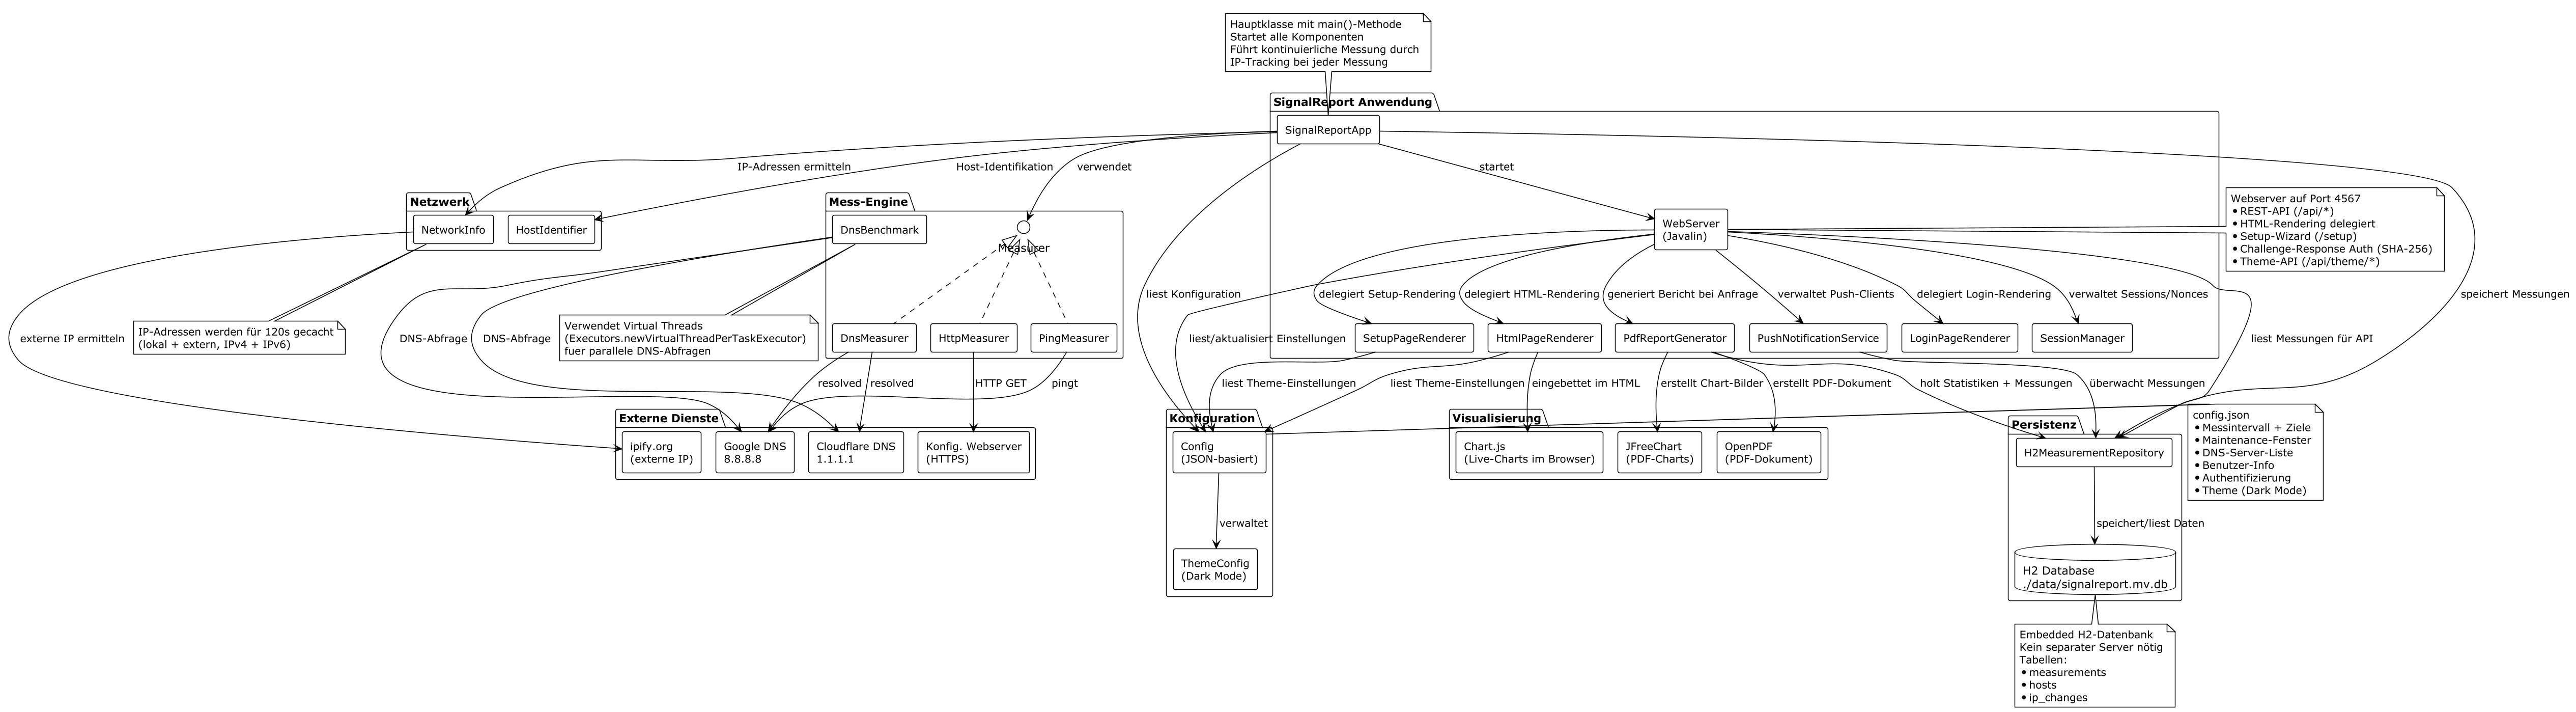
\includegraphics[width=\textwidth]{../diagrams/component-diagram.png}
    \caption{Vollständiges Komponenten-Diagramm}
\end{figure}

\subsection{Sequenz-Diagramm: Messungsablauf}
\begin{figure}[H]
    \centering
    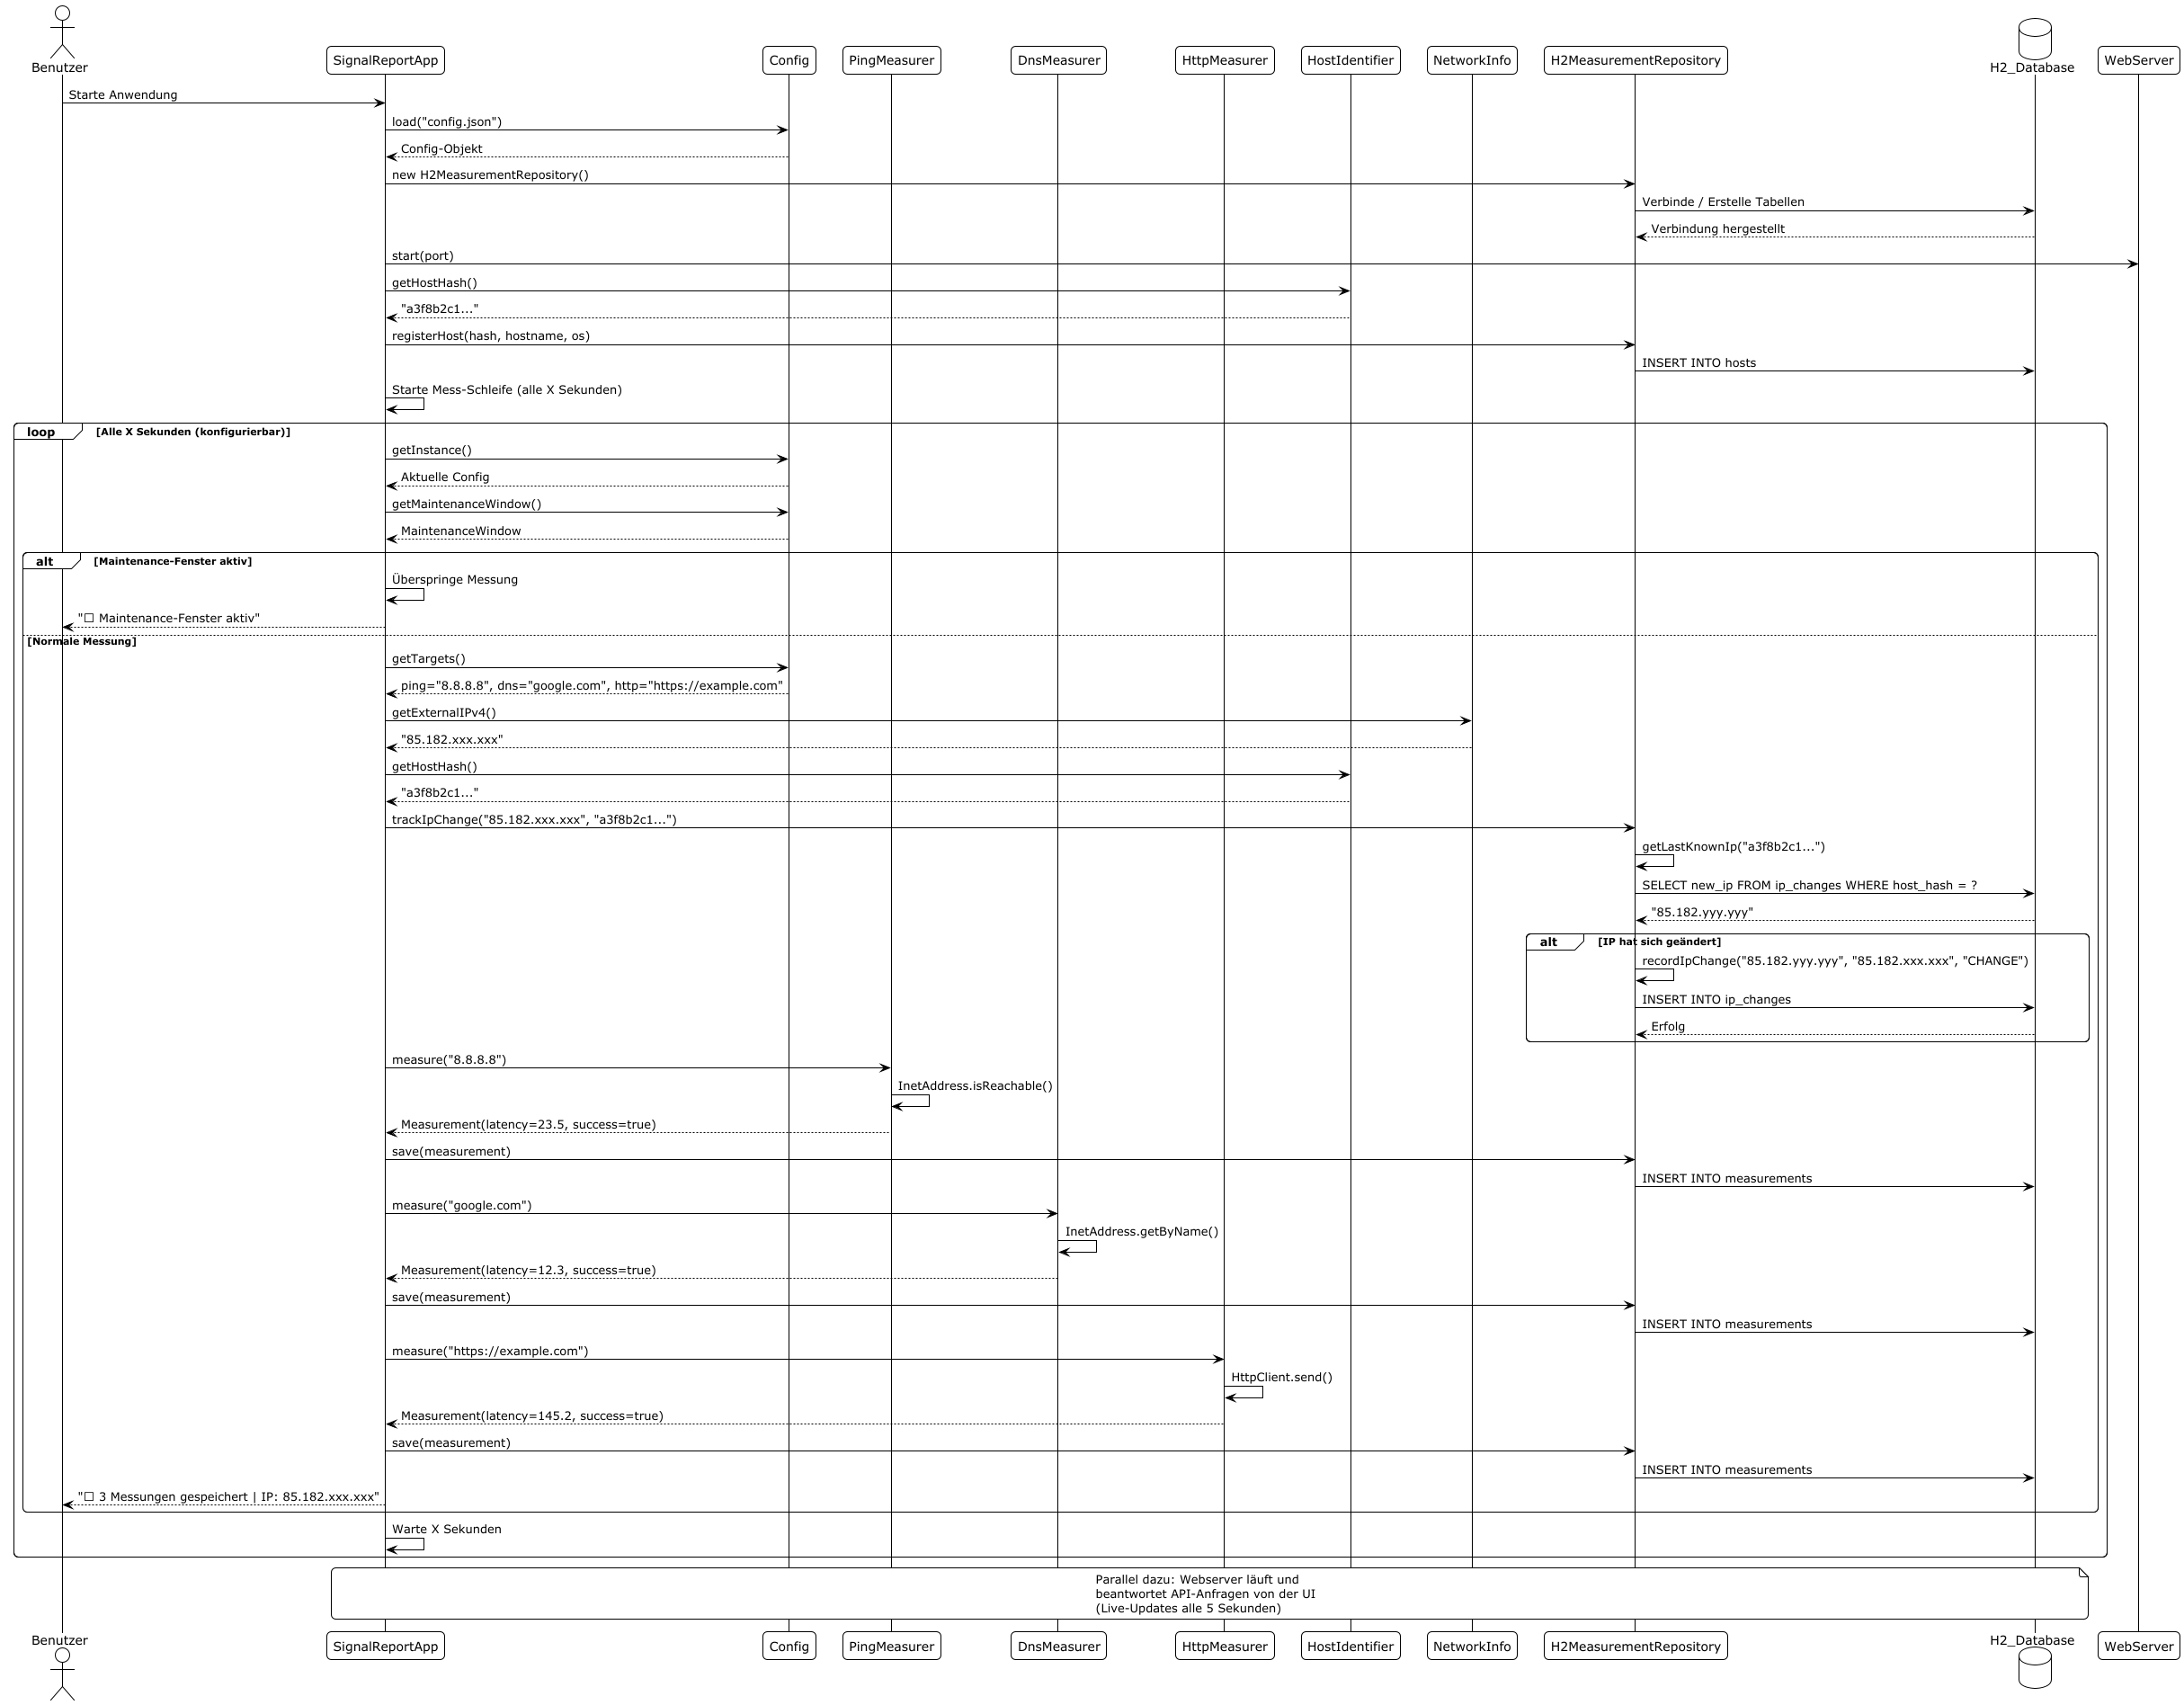
\includegraphics[width=\textwidth]{../diagrams/sequence-measurement.png}
    \caption{Vollständiges Sequenz-Diagramm Messungsablauf}
\end{figure}

\subsection{Sequenz-Diagramm: PDF-Export}
\begin{figure}[H]
    \centering
    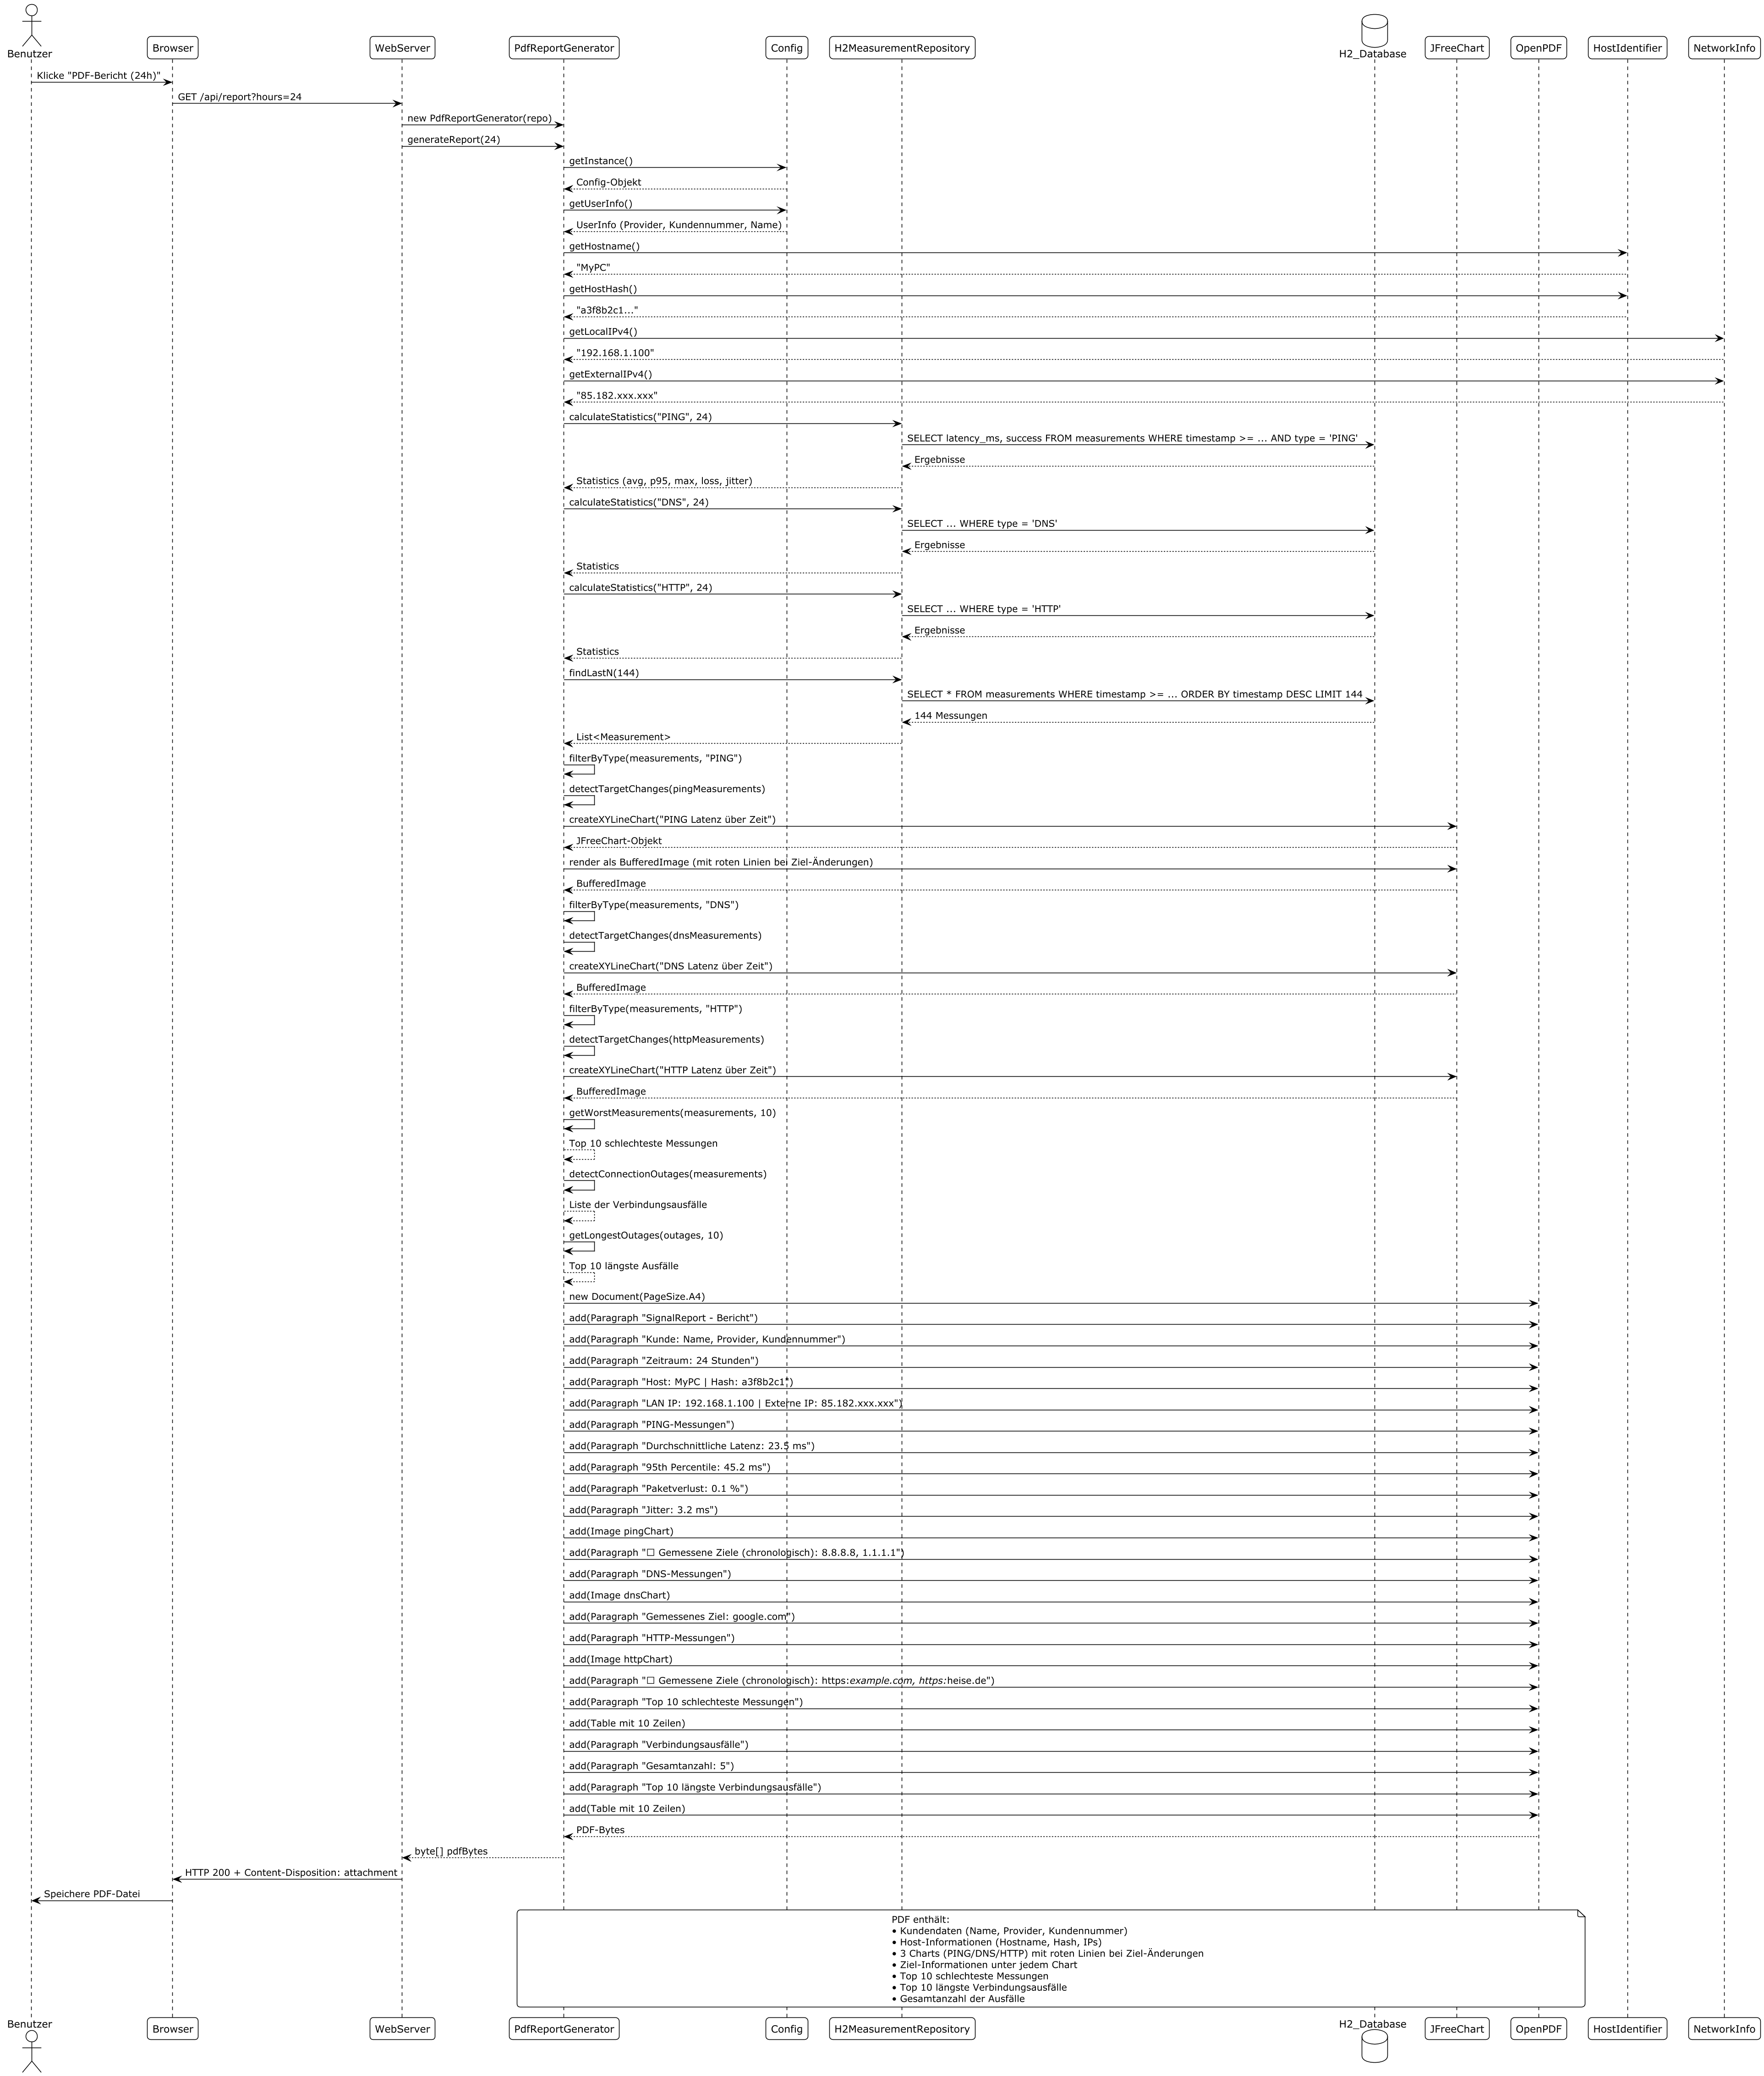
\includegraphics[width=\textwidth]{../diagrams/sequence-pdf.png}
    \caption{Vollständiges Sequenz-Diagramm PDF-Export}
\end{figure}

\subsection{Use-Case-Diagramm}
\begin{figure}[H]
    \centering
    
\includegraphics[width=0.9\textwidth]{../diagrams/usecase-diagram.png}
    \caption{Vollständiges Use-Case-Diagramm}
\end{figure}

\subsection{Deployment-Diagramm}
\begin{figure}[H]
    \centering
    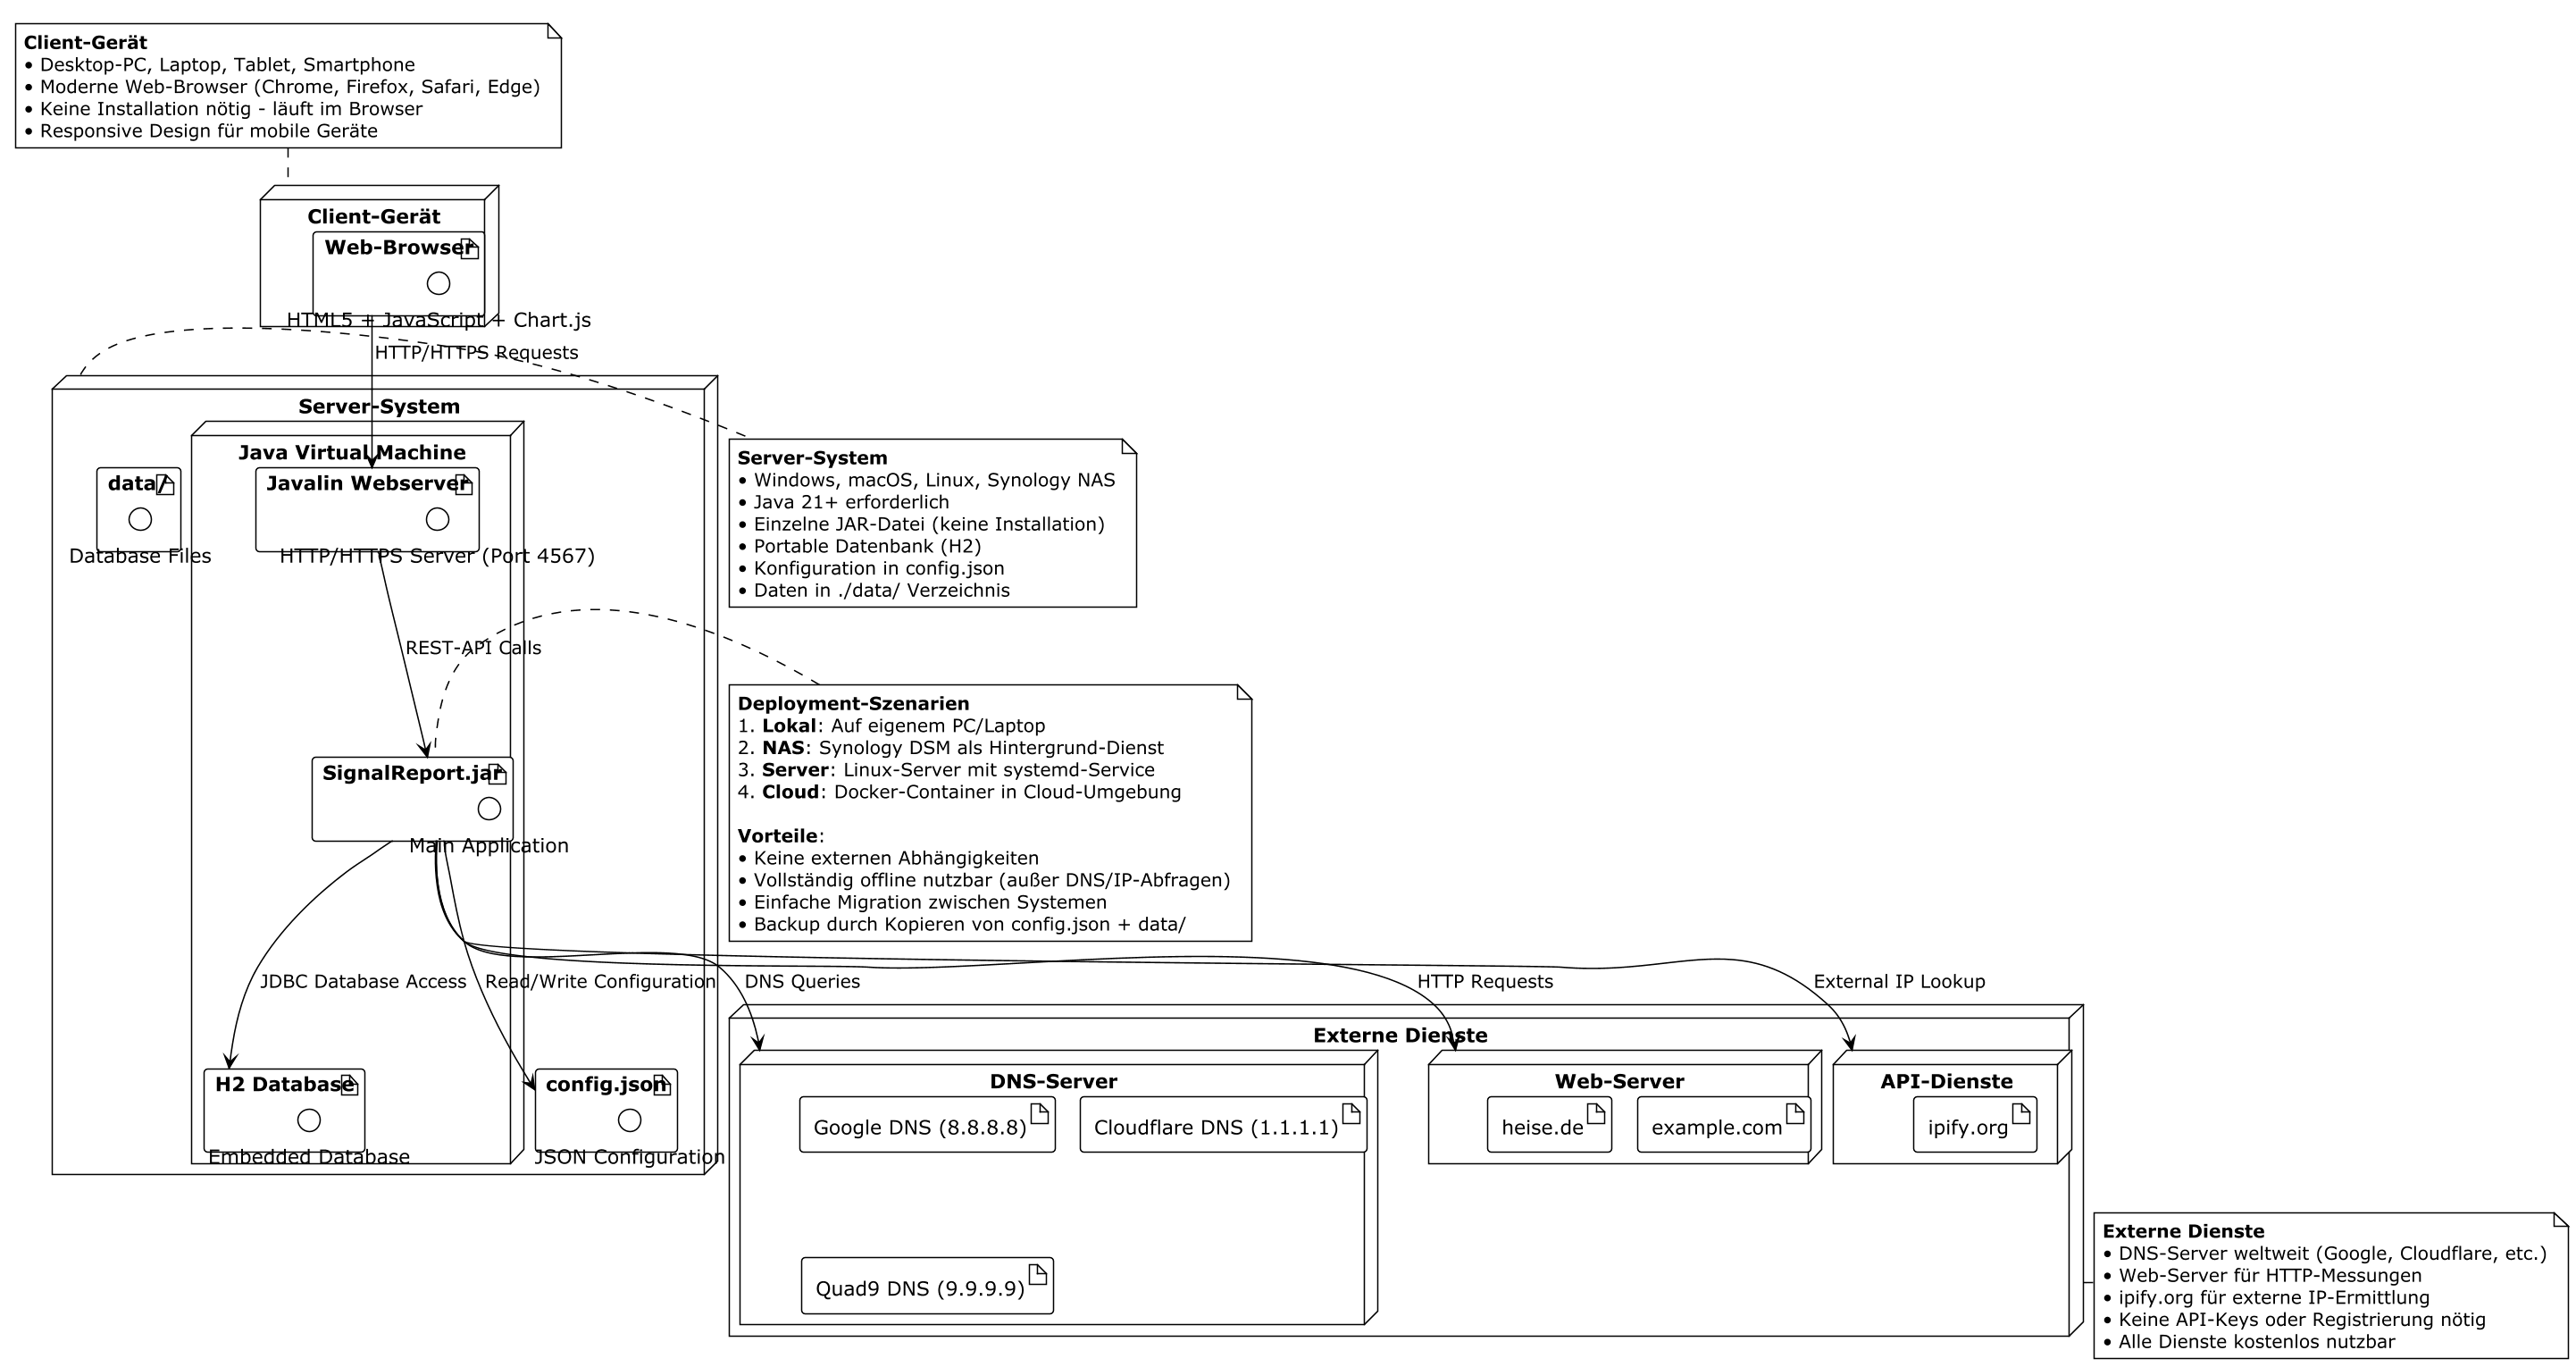
\includegraphics[width=0.9\textwidth]{../diagrams/deployment-diagram.png}
    \caption{Vollständiges Deployment-Diagramm}
\end{figure}

\subsection{State-Diagramm: Authentifizierung}
\begin{figure}[H]
    \centering
    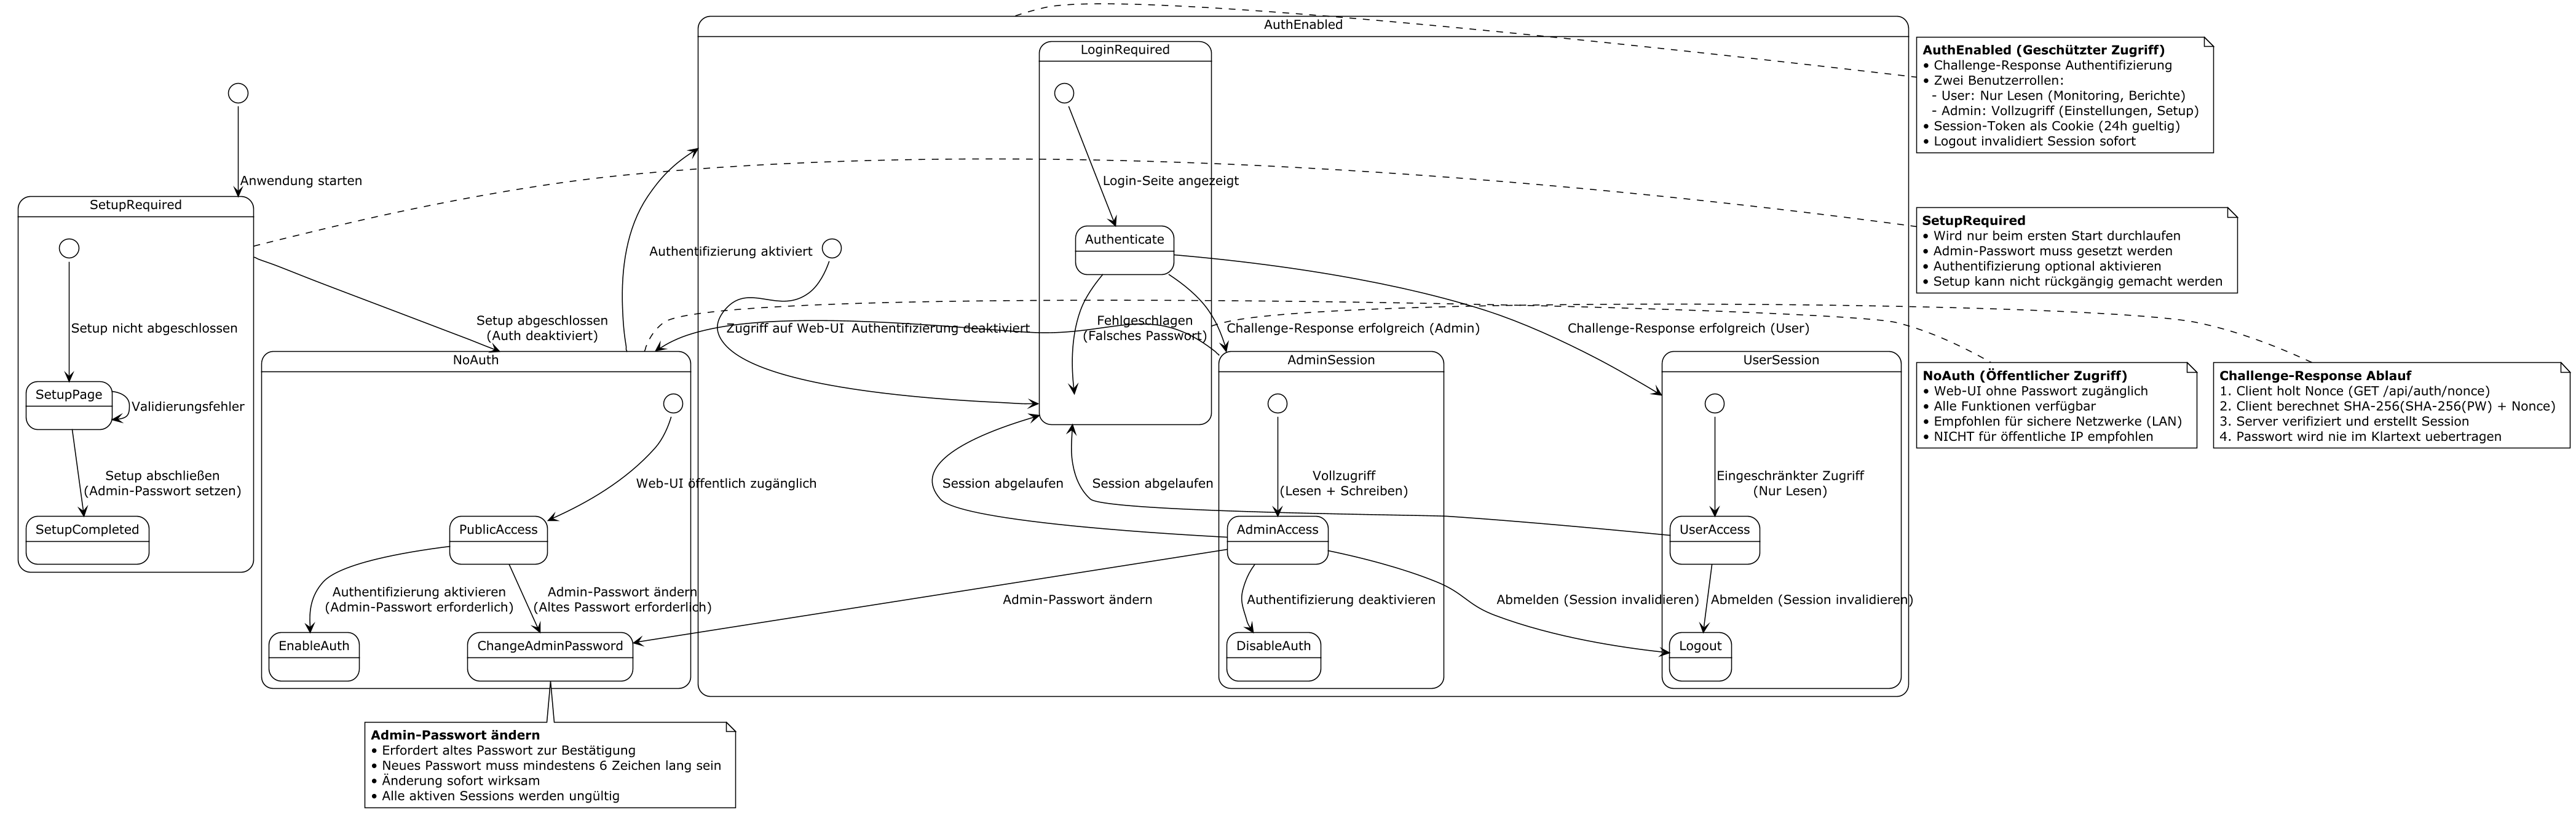
\includegraphics[width=0.9\textwidth]{../diagrams/state-diagram-auth.png}
    \caption{Vollständiges State-Diagramm Authentifizierung}
\end{figure}

% Literaturverzeichnis
\bibliographystyle{plain}
\bibliography{literatur}

\end{document}
